%------------------------------------------------------------------------------
% CHAPTER 4: FORMAL ANALYSIS USING ALLOY
%------------------------------------------------------------------------------
\chapter{Formal Analysis Using Alloy}
\label{ch:alloy}

\section{Alloy's analysis objective}
\label{sec:alloy_intro}

\noindent
In this section, a presentation of the formal modelling activity, conducted using the Alloy formal notation, is provided. The main goal of this activity is to formally describe the domain entities and constraints related to the BBP \emph{trip publication} and \emph{data merging} mechanisms. In particular, we model the lifecycles of manual and automatic trips, the validation of detected obstacles before publication, and the evolution of public paths whose status is updated by aggregating concurrent publications through voting rules. The model is then analyzed through bounded executions and assertion checks to identify inconsistencies and prevent invalid evolutions.

\section{Model Description}
\noindent
The model focuses on the core BBP entities \texttt{RegisteredUser}, \texttt{Trip} (specialized into \texttt{ManualTrip} and \texttt{AutomaticTrip}), \texttt{Path}, and \texttt{Obstacle}, and on the main relations among them, such as how a user records a trip and how that trip contributes to a public path.

\noindent
To correctly capture the \emph{Data Merging} requirement, we introduced the \texttt{Publication} and the global \texttt{PubLog} signatures. They allow us to model the persistence of anonymized data: even if a user later deletes a private trip, its anonymized contribution remains available for public aggregation, so that path status updates are based on the full history of publishable data.

\noindent
Key aspects of the model include:
\begin{itemize}
    \item \textbf{Trip lifecycles.} \texttt{ManualTrip} follows a simpler progression from private creation to optional publication and deletion. \texttt{AutomaticTrip} follows a richer progression, including phases for detecting biking activity, recording, post-processing, and the publication decision, and it may require user validation before becoming publishable.
    \item \textbf{Obstacle validation.} Obstacles are generated from \texttt{AutomaticTrip}s and evolve from detection to validation. The model ensures that an \texttt{AutomaticTrip} cannot be published while it still has any \texttt{Pending} obstacle, reflecting the requirement that false positives must be resolved before data becomes public.
    \item \textbf{Path lifecycle and status aggregation.} A \texttt{Path} becomes public when the first publication about it appears, and subsequent publications trigger the merging phase. The model formalizes the status update logic used by BBP when multiple publications arrive in the same timeframe, including unanimity, majority voting, and tie-breaking rules, while also handling the absorbing nature of the \texttt{PermanentlyClosed} status.
\end{itemize}

\noindent
Physical details such as raw GPS coordinates, accelerometer readings, and external Weather Service interactions are abstracted away, since the goal of this Alloy model is to validate the logical consistency of publishing, validation constraints, and status aggregation rather than low-level data acquisition.




\section{Alloy Code}
\label{sec:alloy_code}

\begin{lstlisting}[language=alloy, caption=BBP Formal Model]
module bbp_formal


// ENUMERATIONS

// Track the lifecycle of a Public Path
enum PathStatus {
  Undefined, Optimal, Medium, Sufficient, RequiresMaintenance, PermanentlyClosed
}

// Track the lifecycle of a Path
enum PathLifecycle {
  NonExistent, Created, MergeData
}

// Track the lifecycle of a manually-recorded Trip
enum ManualTripState {
  mInsertingStreet, mSavedPrivate, mReadyToPublish, mPublished, mDeleted
}

// Track the lifecycle of an automatic-recorded Trip
enum AutomaticTripState {
  aIdle, aDetectBiking, aRecording, aAnalysis, aSavedPrivate, aAwaitingValidation, aReadyToPublish, aNotPublishable, aPublished, aDeleted
}

// Track the lifecycle of an Obstacle
enum ObstacleStatus {
  oNonExistent, Pending, Confirmed, Rejected
}

// SIGNATURES

// Represents one of the Users interacting with BBP
sig User {}  // Guest or Registered

sig RegisteredUser in User {  // Registered users are a subset of all users
  recorded: set Trip
}

// Represents a public Path whose status evolves over time
sig Path {
  var lifecycle: one PathLifecycle,
  var status: one PathStatus
}

// Represents a biking Trip recorded by a Registered User
// Abstract class: subtypes define distinct way of recording the Trip (Manual vs. Automatic)
abstract sig Trip {
  owner: one RegisteredUser,          // The user who generate this data (must be Registered)
  about: one Path,                    // The physical trajectory (Path) this specific trip covers
  reportedStatus: one PathStatus      // The status of the trajectory reported by the User (used in merge)
}

sig ManualTrip extends Trip {
  var mState: one ManualTripState
}

sig AutomaticTrip extends Trip {
  var aState: one AutomaticTripState
}

// Represents a potential anomaly detected by sensors during an Automatic Trip that requires validation
sig Obstacle {
  trip: one AutomaticTrip,
  var oStatus: one ObstacleStatus
}

// Represents the Publication event of a Trip.
sig Publication {
  source: one Trip,
  path: one Path,
  status: one PathStatus
}

// Represents the public, anonymized data used for Path merging (global container of all the publications).
// In this way Trip contribution is never removed, even if the original Trip is later deleted.
one sig PubLog {
  var entries: set Publication
}

// PUBLICATION FACTS AND FUNCTIONS

// Data Consistency: ensures that a Publication accurately reflect the source Trip's data.
fact publicationFieldsConsistent {
  all e: Publication | e.path = e.source.about and e.status = e.source.reportedStatus
}

// Uniqueness: a Trip can generate at most one publication event (no republishing).
fact atMostOnePublicationPerTrip {
  all t: Trip | lone e: Publication | e.source = t
}

// Helper: retrieves the unique Publication associated with a specific Trip, if any.
fun pubOf[t: Trip]: lone Publication {
  { e: Publication | e.source = t }
}

// Publishing trigger: if a Trip is currently in Published, then a corresponding Publication (and PubLog) exists.
// If the Trip is Deleted later, the relative log (PubLog) still remains.
fact publicationCreatedWhenPublished {
  always (all mt: ManualTrip |
    mt.mState = mPublished implies some e: Publication | e.source = mt and e in PubLog.entries
  )
  always (all at: AutomaticTrip |
    at.aState = aPublished implies some e: Publication | e.source = at and e in PubLog.entries
  )
}

// Integrity: a Publication entry exists in the log only if its source Trip
// has reached the 'Published' state at some point in time.
fact noPublicationWithoutPublishing {
  always (all t: Trip |
    (pubOf[t] in PubLog.entries) implies once (
      (t in ManualTrip and t.(ManualTrip <: mState) = mPublished) or
      (t in AutomaticTrip and t.(AutomaticTrip <: aState) = aPublished)
    )
  )
}

// Helper: identifies Publications that have been added to the log in the current time step.
// Used to trigger immediate updates to the Path status.
fun newPublicationsNow[p: Path]: set Publication {
  { e: PubLog.entries | e.path = p and not before (e in PubLog.entries) }
}

// Predicate True if a Path has received new data updates in the current step.
pred somePublicationNow[p: Path] {
  some newPublicationsNow[p]
}

// Persistence: the Publication Log is monotonic; entries are never removed.
// Once an anonymized contribution exists, it stays, even if the original user deletes their Trip.
fact publicationLogIsMonotone {
  always (all e: Publication |
    (e in PubLog.entries) implies after (e in PubLog.entries)
  )
}

// USER AND TRIP OWNERSHIP FACTS

// Ensures that all Trips are recorded by exactly one Registered User and the 'recorded' matches that ownership
fact recordedMatchesOwner {
  all t: Trip | t in t.owner.recorded
  all u: RegisteredUser | u.recorded = { t: Trip | t.owner = u }
}

// Ensures that a RegisteredUser does not have two concurrent AutomaticTrips in critical "active" phases.
fact oneActiveAutomaticTripPerUser {
  always (all u: RegisteredUser |
    lone at: AutomaticTrip |
      at.owner = u and at.aState in (aDetectBiking + aRecording)
  )
}

// Ensures correct Initial State
fact initStates {
  all mt: ManualTrip | not before (mt.mState = mInsertingStreet)
  all at: AutomaticTrip | not before (at.aState = aIdle)
  all o: Obstacle | not before (o.oStatus = oNonExistent)
  no PubLog.entries and not before (no PubLog.entries)
}

// OBSTACLE LIFECYCLE

// Ensures that the lifecycle of an Obstacle follows the correct sequence
fact obstacleLifecycle {
  all o: Obstacle |
    // 1. Initial State (NonExistent)
    once (o.oStatus = oNonExistent)
    and

    // 2. Creation: NonExistent -> Pending
    // This happens only when the associated trip is in Analysis
    always (
      o.oStatus = oNonExistent implies
      (
        // Stays NonExistent
        after (o.oStatus = oNonExistent)
        or
        // or becomes Pending (when detected)
        (after (o.oStatus = Pending) and o.trip.aState = aAnalysis)
      )
    )
    and

    // 3. Validation: Pending -> Confirmed/Rejected
    // This happens when the trip is AwaitingValidation
    always (
      o.oStatus = Pending implies
      eventually (o.oStatus = Confirmed or o.oStatus = Rejected)
    )
    and

    // 4. Final States are absorbing
    always (
      o.oStatus in (Confirmed + Rejected) implies o.oStatusI = o.oStatus
    )
}

// MANUAL TRIP LIFECYCLE

// Ensures that the states of a ManualTrip lifecycle are in the correct sequence:
fact manualTripStatus {
  all mt: ManualTrip |
    // 1. Initial State: must start at InsertingStreet
    once (mt.mState = mInsertingStreet)
    and

    // 2. InsertingStreet -> SavedPrivate
    always (
      mt.mState = mInsertingStreet implies
      eventually (mt.mState = mSavedPrivate)
    )
    and

    // 3. SavedPrivate -> ReadyToPublish OR Deleted
    always (
      mt.mState = mSavedPrivate implies (
        once (mt.mState = mInsertingStreet) and
        eventually (mt.mState = mReadyToPublish or mt.mState = mDeleted)
      )
    )
    and

    // 4. ReadyToPublish -> Published OR Deleted
    always (
      mt.mState = mReadyToPublish implies (
        once (mt.mState = mSavedPrivate) and
        eventually (mt.mState = mPublished or mt.mState = mDeleted)
      )
    )
    and

    // 5. Published -> Deleted
    always (
      mt.mState = mPublished implies (
        once (mt.mState = mReadyToPublish) and
        eventually (mt.mState = mDeleted)
      )
    )
    and

    // 6. Deleted is an absorbing state
    always (
      mt.mState = mDeleted implies
      once (mt.mState = mSavedPrivate or mt.mState = mReadyToPublish or mt.mState = mPublished)
    )
}

// AUTOMATIC TRIP LIFECYCLE

// Ensures that the states of an AutomaticTrip lifecycle are in the correct sequence:
fact automaticTripStatus {
  all at: AutomaticTrip |
    // 1. Initial State
    once (at.aState = aIdle)
    and

    // 2. Idle -> DetectBiking
    always (
      at.aState = aIdle implies
      eventually (at.aState = aDetectBiking)
    )
    and

    // 3. DetectBiking -> Recording (Loop entry)
    always (
      at.aState = aDetectBiking implies (
        once (at.aState = aIdle or at.aState = aRecording) and
        eventually (at.aState = aRecording)
      )
    )
    and

    // 4. Recording -> DetectBiking (Loop) OR Analysis (Progress)
    always (
      at.aState = aRecording implies (
        once (at.aState = aDetectBiking) and
        eventually (at.aState = aDetectBiking or at.aState = aAnalysis)
      )
    )
    and

    // 5. Analysis -> SavedPrivate
    always (
      at.aState = aAnalysis implies (
        once (at.aState = aRecording) and
        eventually (at.aState = aSavedPrivate)
      )
    )
    and

    // 6. SavedPrivate -> ReadyToPublish OR AwaitingValidation OR Deleted
    always (
      at.aState = aSavedPrivate implies (
        once (at.aState = aAnalysis) and
        eventually (at.aState = aReadyToPublish or at.aState = aAwaitingValidation or at.aState = aDeleted)
      )
    )
    and

    // 7. AwaitingValidation -> ReadyToPublish OR NotPublishable OR Deleted
    always (
      at.aState = aAwaitingValidation implies (
        once (at.aState = aSavedPrivate) and
        eventually (at.aState = aReadyToPublish or at.aState = aNotPublishable or at.aState = aDeleted)
      )
    )
    and

    // 8. ReadyToPublish -> Published OR Deleted
    always (
      at.aState = aReadyToPublish implies (
        once (at.aState = aSavedPrivate or at.aState = aAwaitingValidation) and
        eventually (at.aState = aPublished or at.aState = aDeleted)
      )
    )
    and

    // 9. Published -> Deleted
    always (
      at.aState = aPublished implies (
        once (at.aState = aReadyToPublish) and
        eventually (at.aState = aDeleted)
      )
    )
    and

    // 10. Deleted is absorbing
    always (
      at.aState = aDeleted implies
      once (at.aState != aDeleted)
    )

  // AwaitingValidation means that exists at least one pending obstacle
  always (
    all at: AutomaticTrip |
      at.aState = aAwaitingValidation
      implies some o: Obstacle | o.trip = at and o.oStatus = Pending
  )

  // ReadyToPublish means there are no pending obstacles
  // (If no obstacles were detected at all, this is also satisfied)
  always (
    all at: AutomaticTrip |
      at.aState = aReadyToPublish
      implies no o: Obstacle | o.trip = at and o.oStatus = Pending
  )

  // NotPublishable means some obstacle is still pending (validation not completed).
  always (
    all at: AutomaticTrip |
      at.aState = aNotPublishable
      implies some o: Obstacle | o.trip = at and o.oStatus = Pending
  )

  // Once NotPublishable, it can never become Published.
  always (all at: AutomaticTrip |
    at.aState = aNotPublishable implies after always (at.aState != aPublished)
  )

  // User must validate within a time interval, otherwise NotPublishable.
  // We model: if AwaitingValidation persists without resolving pending obstacles, then eventually the trip can become NotPublishable.
  always (all at: AutomaticTrip |
    (at.aState = aAwaitingValidation)
    implies eventually (at.aState = aReadyToPublish or at.aState = aNotPublishable)
  )
}

// PATH LIFECYCLE + STATUS EVOLUTION

// first publication --> Created
// later publications --> MergeData

// Helper: were there publications for a given Path before?
pred hadPublicationBefore[p: Path] {
  some e: Publication | e.path = p and before (e in PubLog.entries)
}

fact pathLifecycleCreationVsMerge {
  always (all p: Path |
    some newPublicationsNow[p] implies
      ( (not hadPublicationBefore[p] and p.lifecycle = Created)
        or
        (hadPublicationBefore[p] and p.lifecycle = MergeData)
      )
  )
}

// Ensures that the states of a Path lifecycle are in the correct sequence:
fact pathStatus {
  all p: Path |
    // 1. Initial State: It must have started as NonExistent
    once (p.lifecycle = NonExistent)
    and

    // 2. NonExistent -> Created (happens when first publication arrives)
    always (
      p.lifecycle = NonExistent implies
      after (p.lifecycle = NonExistent or p.lifecycle = Created)
    )
    and

    // 3. Created -> MergeData
    always (
      p.lifecycle = Created implies
      eventually (p.lifecycle = MergeData)
    )
    and

    // 4. MergeData -> MergeData OR PermanentlyClosed
    always (
      p.lifecycle = MergeData implies (
        once (p.lifecycle = Created) and
        eventually (p.lifecycle = MergeData or p.status = PermanentlyClosed)
      )
    )
    and

    // 5. PermanentlyClosed is absorbing
    always (
      p.status = PermanentlyClosed implies
      after always (p.status = PermanentlyClosed)
    )
}

fact pathLifecycleAndStatus {

  // 1. Lifecycle: A Path is public (Created/Merge) IFF it has entries
  always (all p: Path |
    (some e: PubLog.entries | e.path = p) iff (p.lifecycle in Created + MergeData)
  )

  // 1.1 Ensure NonExistent maps to no entries
  always (all p: Path |
    p.lifecycle = NonExistent implies no e: PubLog.entries | e.path = p
  )

  // 1.2 If NonExistent, Status is Undefined
  always (all p: Path |
    p.lifecycle = NonExistent implies p.status = Undefined
  )

  // 3. Merging Logic
  always (all p: Path |
    (p.status != PermanentlyClosed) implies {  // Merge can be applied only when the path is not permanently closed.
      let S = newPublicationsNow[p] |  // Used to detect the number of concurrent Publications for the same Path

      // CASE A: no new publications (S is empty)
      ( #S = 0 implies (
          // If the path exists, keep status
          (p.lifecycle != NonExistent implies p.statusI = p.status)
      ))
      and

      // VOTING LOGIC (applies even if p.lifecycle was NonExistent)

      // CASE B: 1 new publication --> Adopt that status
      ( #S = 1 implies p.statusI = (S.status) )
      and

      // CASE C: 2 new publications --> Unanimity or Keep Previous
      ( #S = 2 implies (
          // Sub-case 1: Unanimity
          (one s: PathStatus | (all e: S | e.status = s) and p.statusI = s)
          or
          // Sub-case 2: Disagreement
          (not (one s: PathStatus | all e: S | e.status = s) implies (
              p.lifecycle != NonExistent implies p.statusI = p.status
              else p.statusI in S.status
          ))
      ))
      and

      // CASE D: 3+ publications --> Majority Voting
      ( #S >= 3 implies (
          // Sub-case 1: Strict Winner Found
          (some s: PathStatus |
             #( {e: S | e.status = s} ) >= 2
             and
             (all other: PathStatus - s | #( {e: S | e.status = s} ) > #( {e: S | e.status = other} ))
             and
             p.statusI = s
          )
          or
          // Sub-case 2: No Winner (tie)
          (not (some s: PathStatus |
             #( {e: S | e.status = s} ) >= 2
             and
             (all other: PathStatus - s | #( {e: S | e.status = s} ) > #( {e: S | e.status = other} ))
            ) implies (
             // Tie-breaking logic: keep the previous status
             p.lifecycle != NonExistent implies p.statusI = p.status
             else p.statusI in S.status
          ))
        )
      )
    }
  )
}
\end{lstlisting}

\subsection{Example 1: Majority voting for Path status update}

\noindent
This example shows three \texttt{ManualTrip}s about the same \texttt{Path} published in the same timeframe (two reporting the status \texttt{Optimal}, and one reporting \texttt{RequiresMaintenance}). The execution illustrates alle the states of the trips recording: when all three become published concurrently, the \texttt{Path} is created and its status is updated according to majority voting, resulting in \texttt{Optimal}. \\In the Alloy model, the \texttt{m} prefix is used only to distinguish \texttt{ManualTrip} statuses from \texttt{AutomaticTrip} ones.
\begin{lstlisting}[language=alloy]
pred majorityMergeUpdatesStatus {
  #RegisteredUser = 3
  #Path = 1
  #ManualTrip = 3
  #AutomaticTrip = 0
  #Obstacle = 0
  #Publication = 3

  one p: Path |

    // Otherwise PermanentlyClosed is absorbing and blocks any update
    always (p.status != PermanentlyClosed) and

    // All trips refer to the same path
    all mt: ManualTrip | mt.about = p and

    // Two report Optimal, one reports RequiresMaintenance
    some disj mt1, mt2, mt3: ManualTrip |
      mt1.reportedStatus = Optimal and
      mt2.reportedStatus = Optimal and
      mt3.reportedStatus = RequiresMaintenance and

    // All become published (so their publications appear in the log)
    eventually (mt1.mState = mPublished and mt2.mState = mPublished and mt3.mState = mPublished) and

    // Eventually the Path is created AND its status reflects the majority 
    eventually (p.lifecycle != NonExistent and p.status = Optimal)
}

run majorityMergeUpdatesStatus for 5 steps
\end{lstlisting}

\begin{figure}[H]
    \centering
    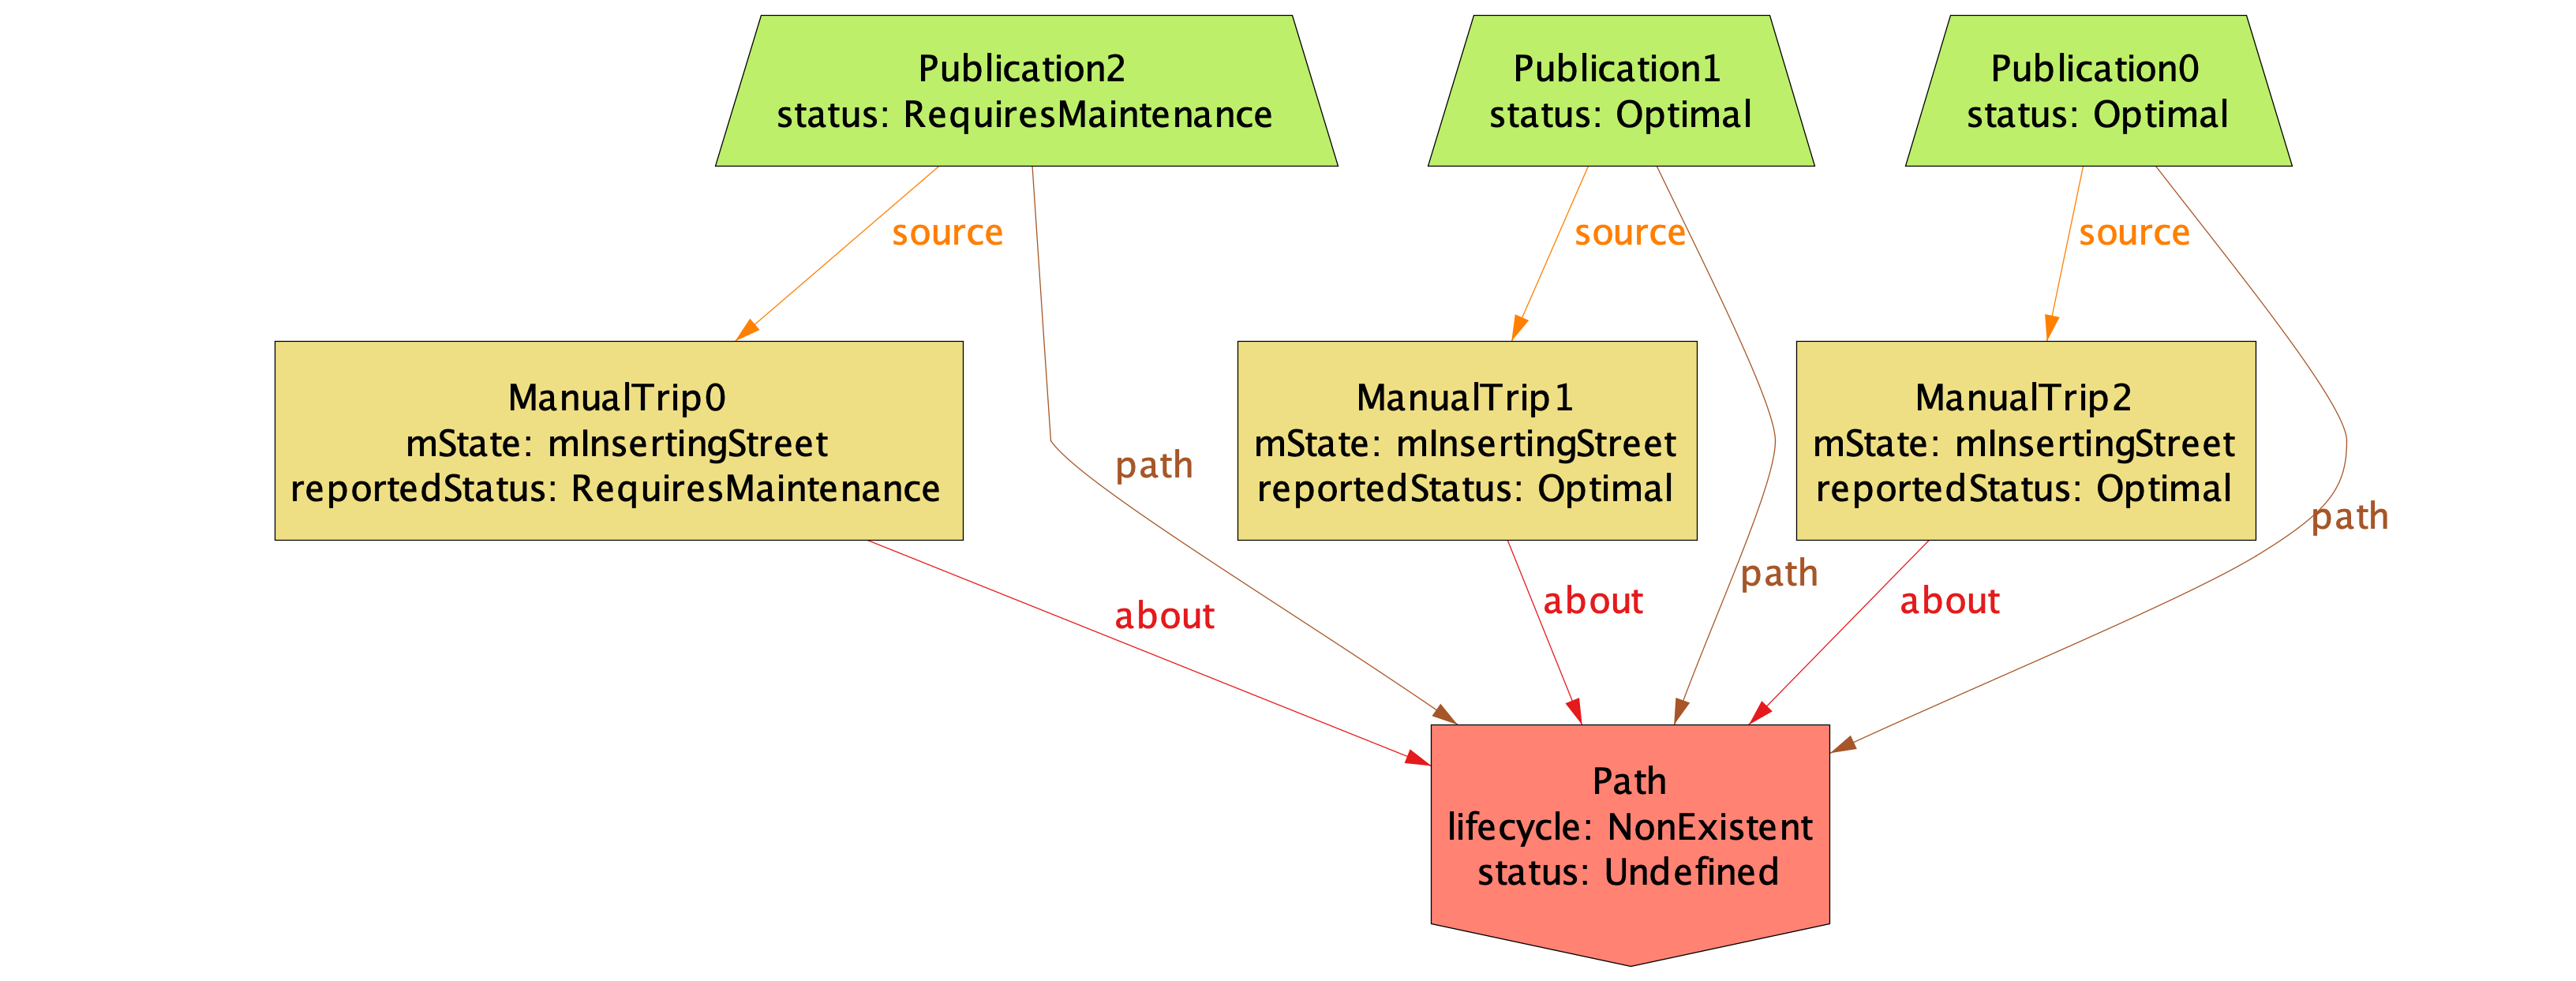
\includegraphics[width=\textwidth]{diagrams/alloy_ex1/alloy_ex1_s0.png}
    \caption{Example 1 evolution: state 0}
    \label{fig:placeholder}
\end{figure}
\begin{figure}[H]
    \centering
    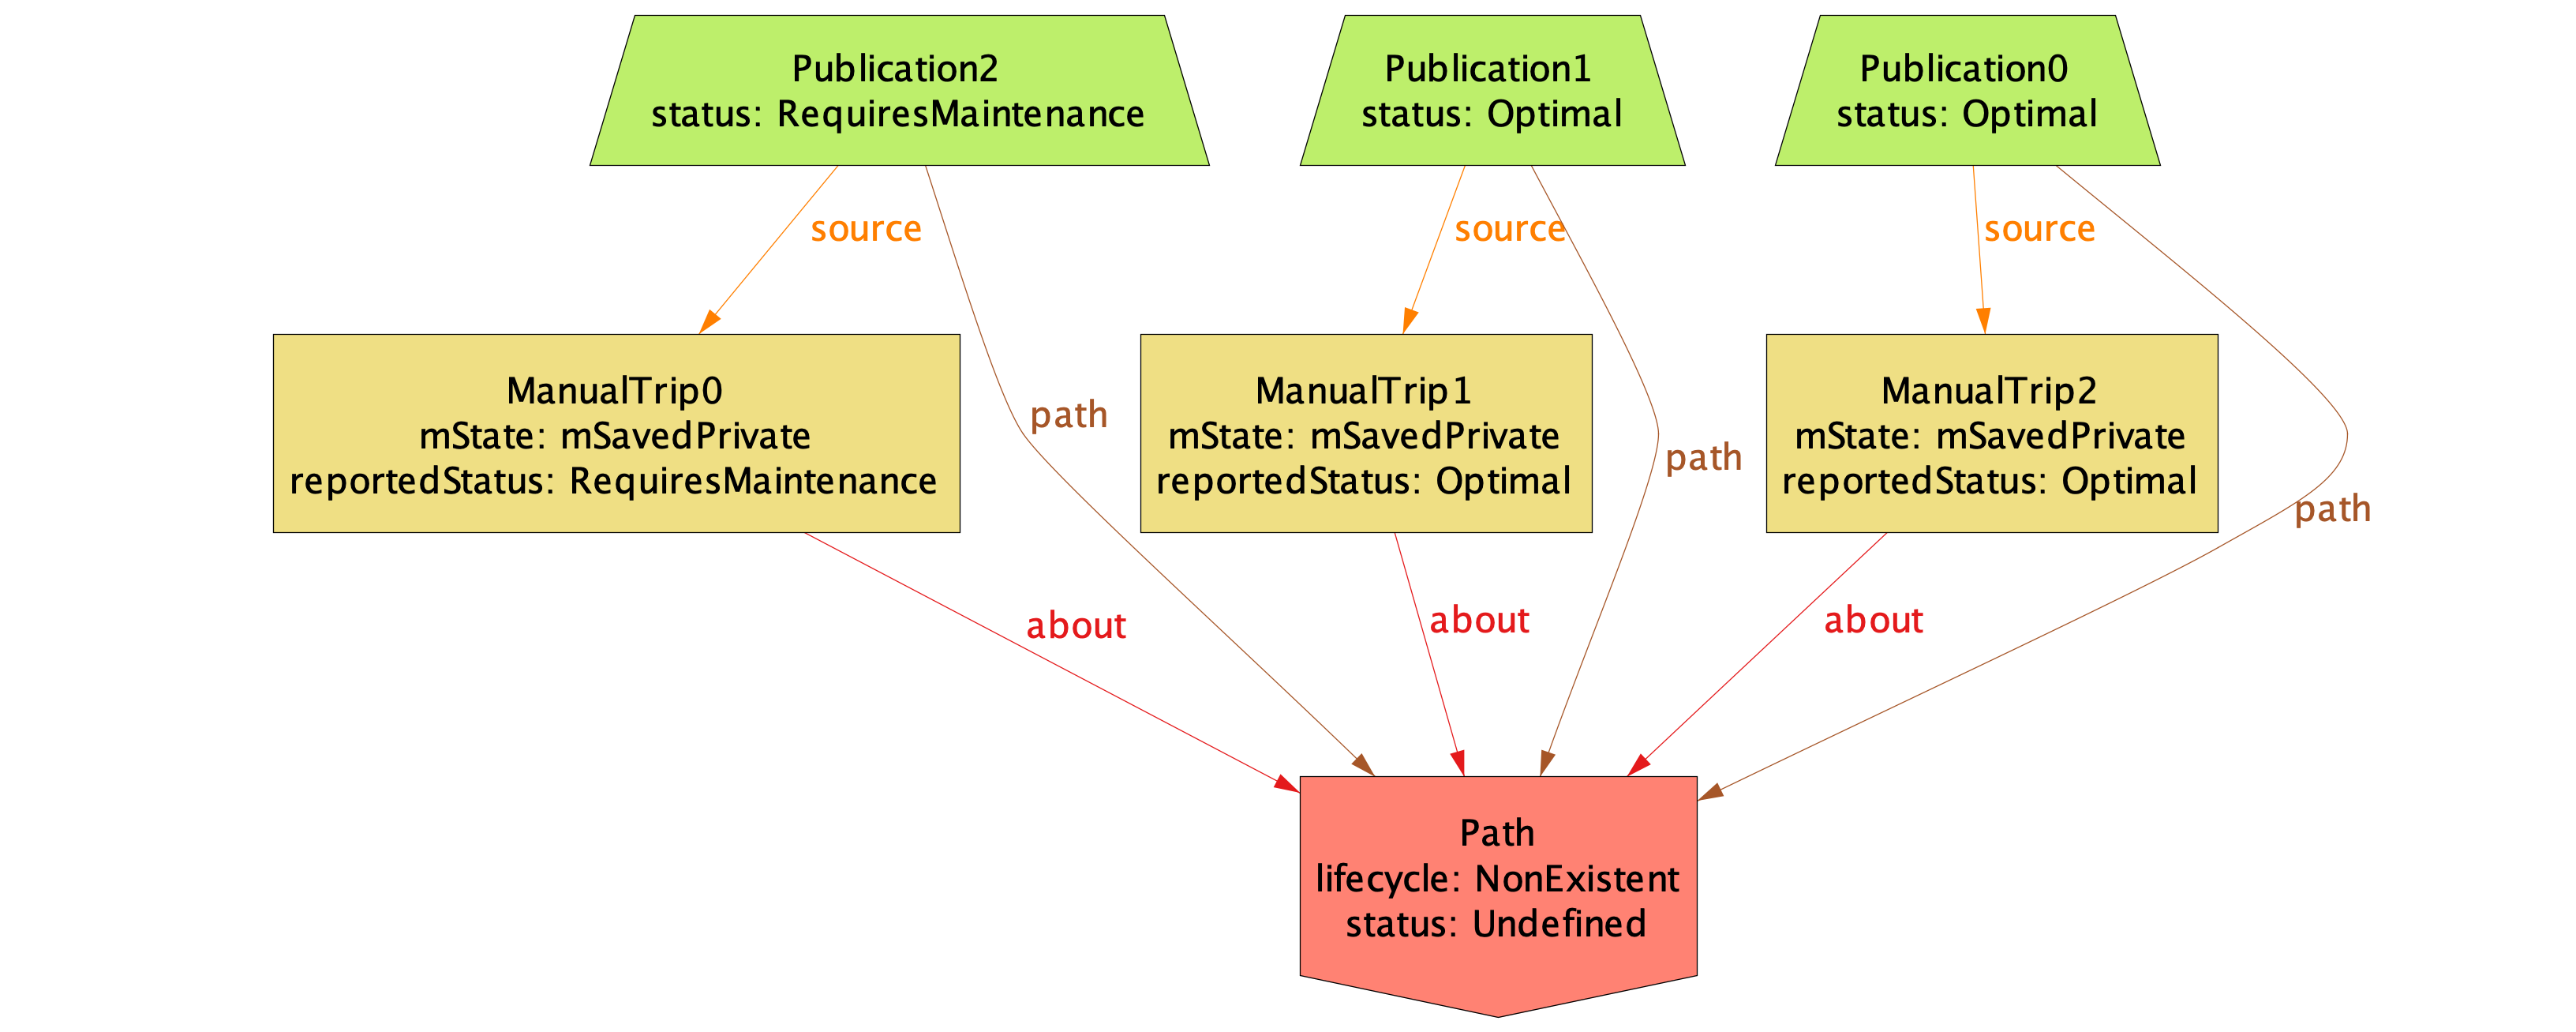
\includegraphics[width=\textwidth]{diagrams/alloy_ex1/alloy_ex1_s1.png}
    \caption{Example 1 evolution: state 1}
    \label{fig:placeholder}
\end{figure}
\begin{figure}[H]
    \centering
    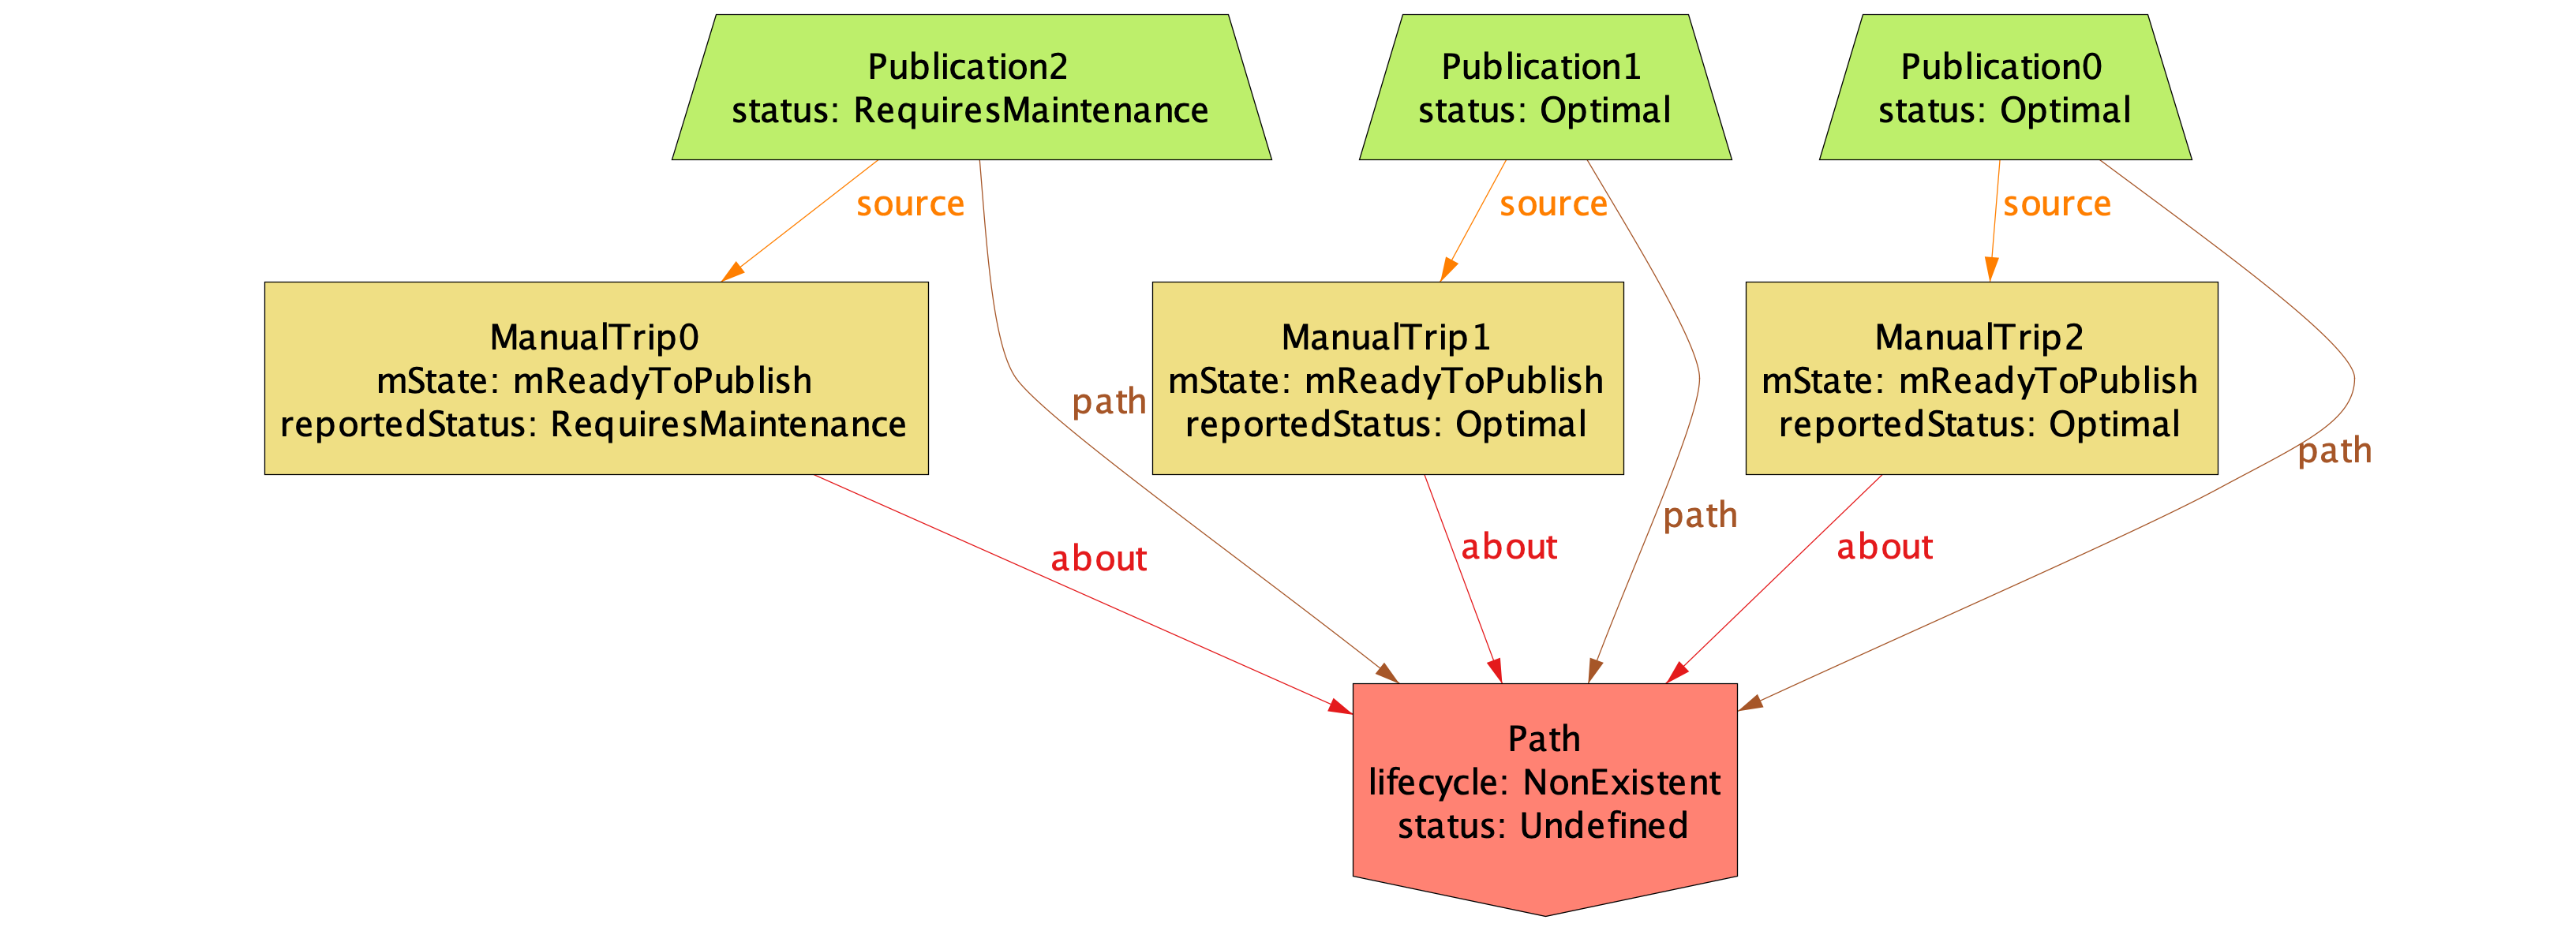
\includegraphics[width=\textwidth]{diagrams/alloy_ex1/alloy_ex1_s2.png}
    \caption{Example 1 evolution: state 2}
    \label{fig:placeholder}
\end{figure}
\begin{figure}[H]
    \centering
    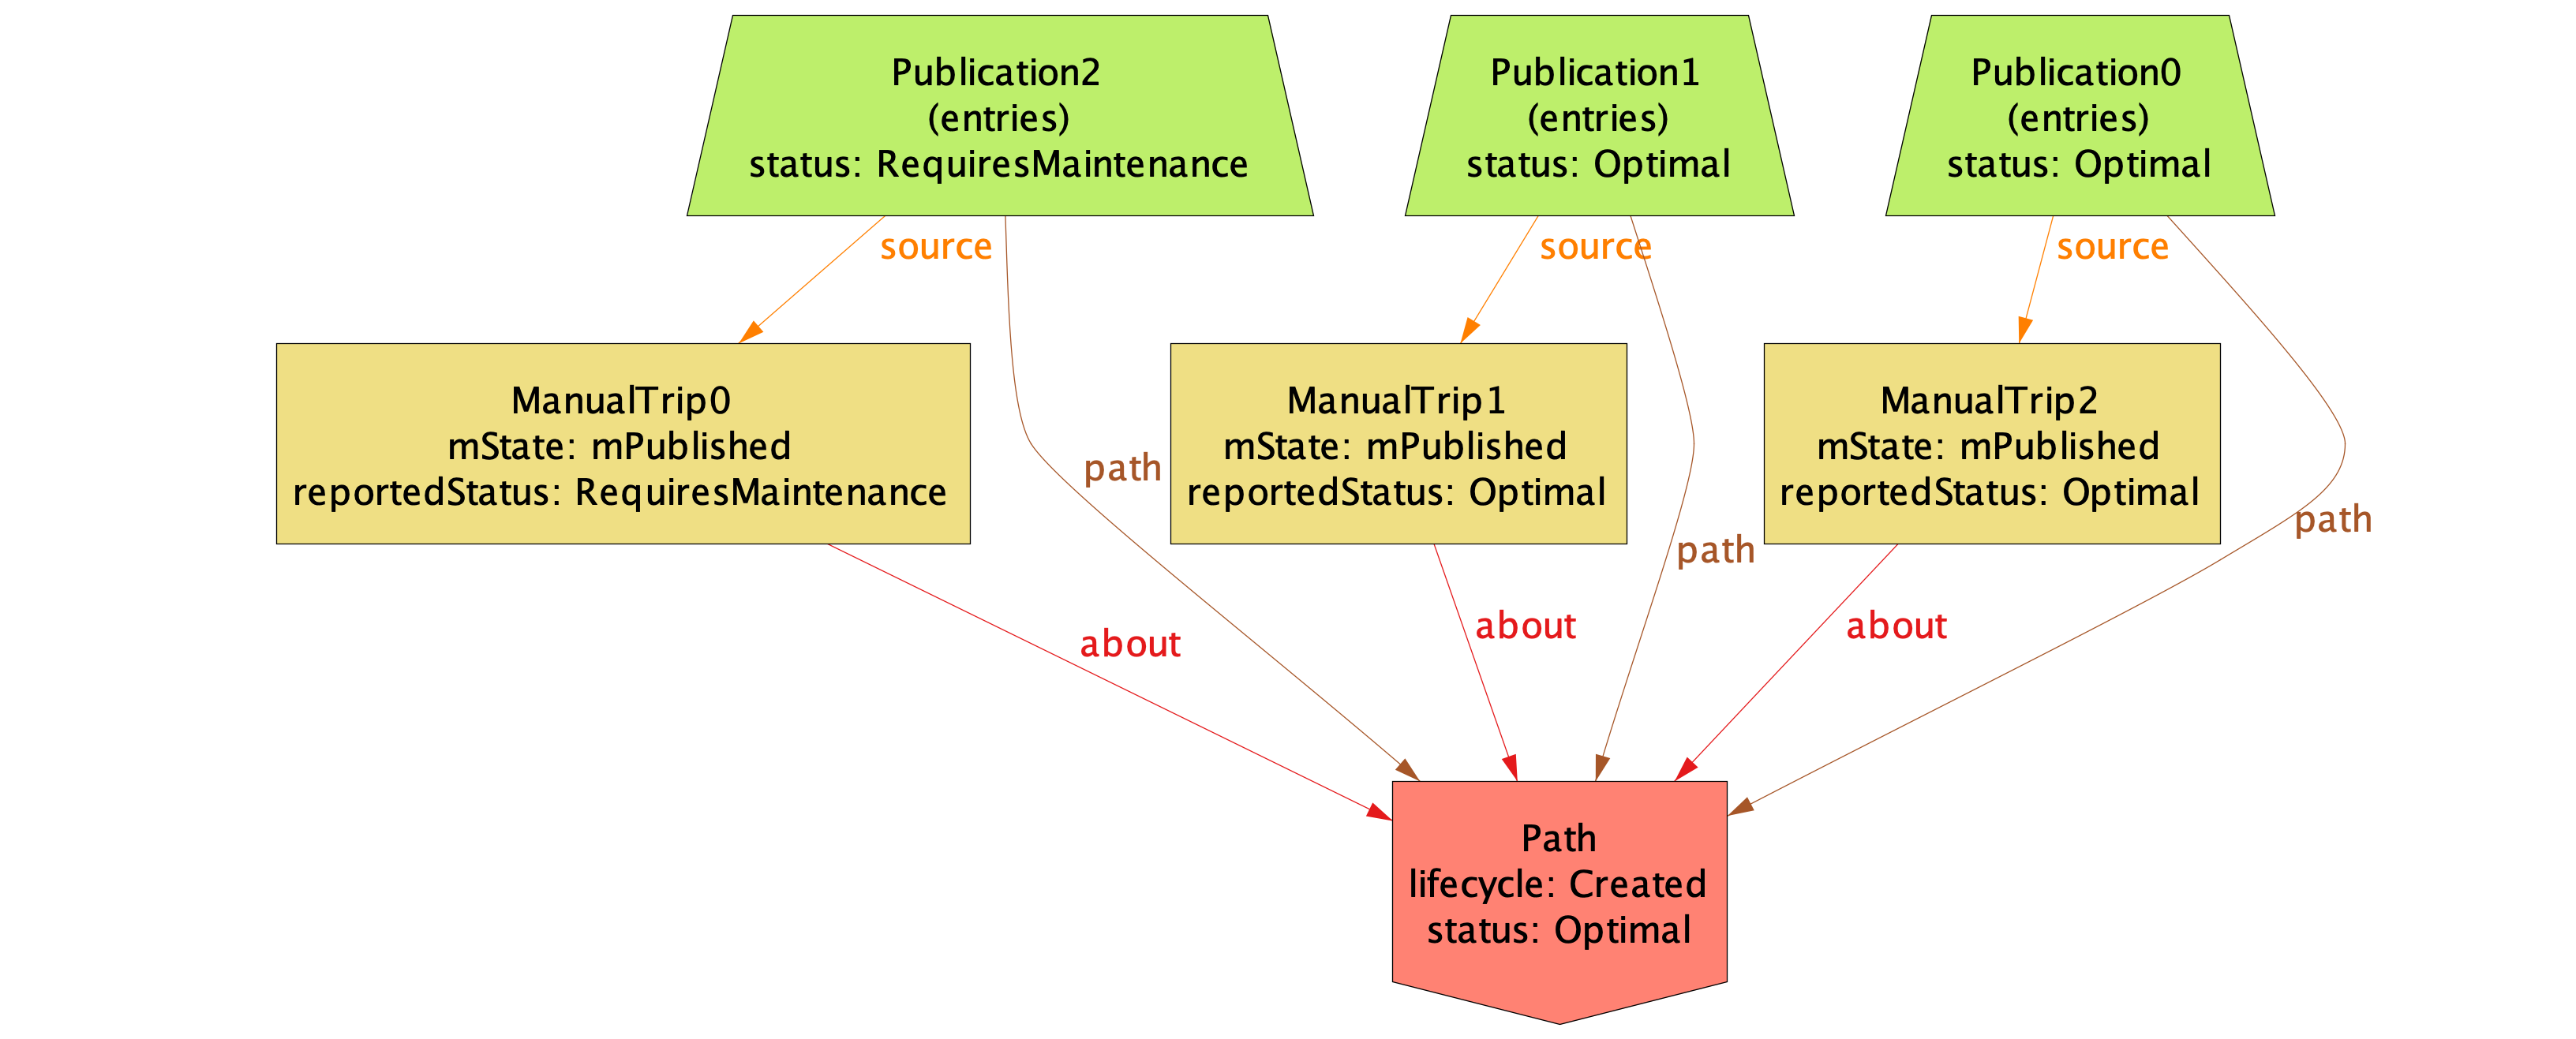
\includegraphics[width=\textwidth]{diagrams/alloy_ex1/alloy_ex1_s3.png}
    \caption{Example 1 evolution: state 3}
    \label{fig:placeholder}
\end{figure}

\subsection{Example 2: Automatic Trip recording \& Obstacle validation}
\noindent

This example shows an \texttt{AutomaticTrip} with a detected \texttt{Obstacle}: the trip reaches \texttt{AwaitingValidation} while the obstacle is \texttt{Pending}, then the user confirms/rejects it, enabling \texttt{ReadyToPublish} and eventually \texttt{Published}. When the \texttt{AutomaticTrip} becomes \texttt{Published}, the respective public Path is created. The execution shows the entire \texttt{AutomaticTrip} recording process and confirms that publication is not possible with pending obstacles. \\In the Alloy model, the \texttt{a} prefix is used only to distinguish \texttt{AutomaticTrip} statuses from \texttt{ManualTrip} ones.
\begin{lstlisting}[language=alloy]
pred autoTripValidationThenPublish {
  
  #RegisteredUser = 1
  #ManualTrip = 0
  #AutomaticTrip = 1
  #Path = 1
  #Publication = 1
  #Obstacle = 1

  one u: RegisteredUser |
  one at: AutomaticTrip |
  one p: Path |
  one o: Obstacle |
  {
    at.owner = u
    at.about = p
    at in u.recorded

    o.trip = at

    // At some point we are awaiting validation --> obstacle must be pending 
    eventually (at.aState = aAwaitingValidation and o.oStatus = Pending)

    // Later the obstacle is no longer pending (confirmed or rejected)
    eventually (o.oStatus = Confirmed or o.oStatus = Rejected)

    // Then the trip can become ready to publish (and, later, published)
    eventually (at.aState = aReadyToPublish)
    eventually (at.aState = aPublished)

    // When published, a publication exists and is in the public log
    eventually (some pubOf[at] and pubOf[at] in PubLog.entries)
  }
}

run autoTripValidationThenPublish for 10
\end{lstlisting}

\begin{figure}[H]
    \centering
    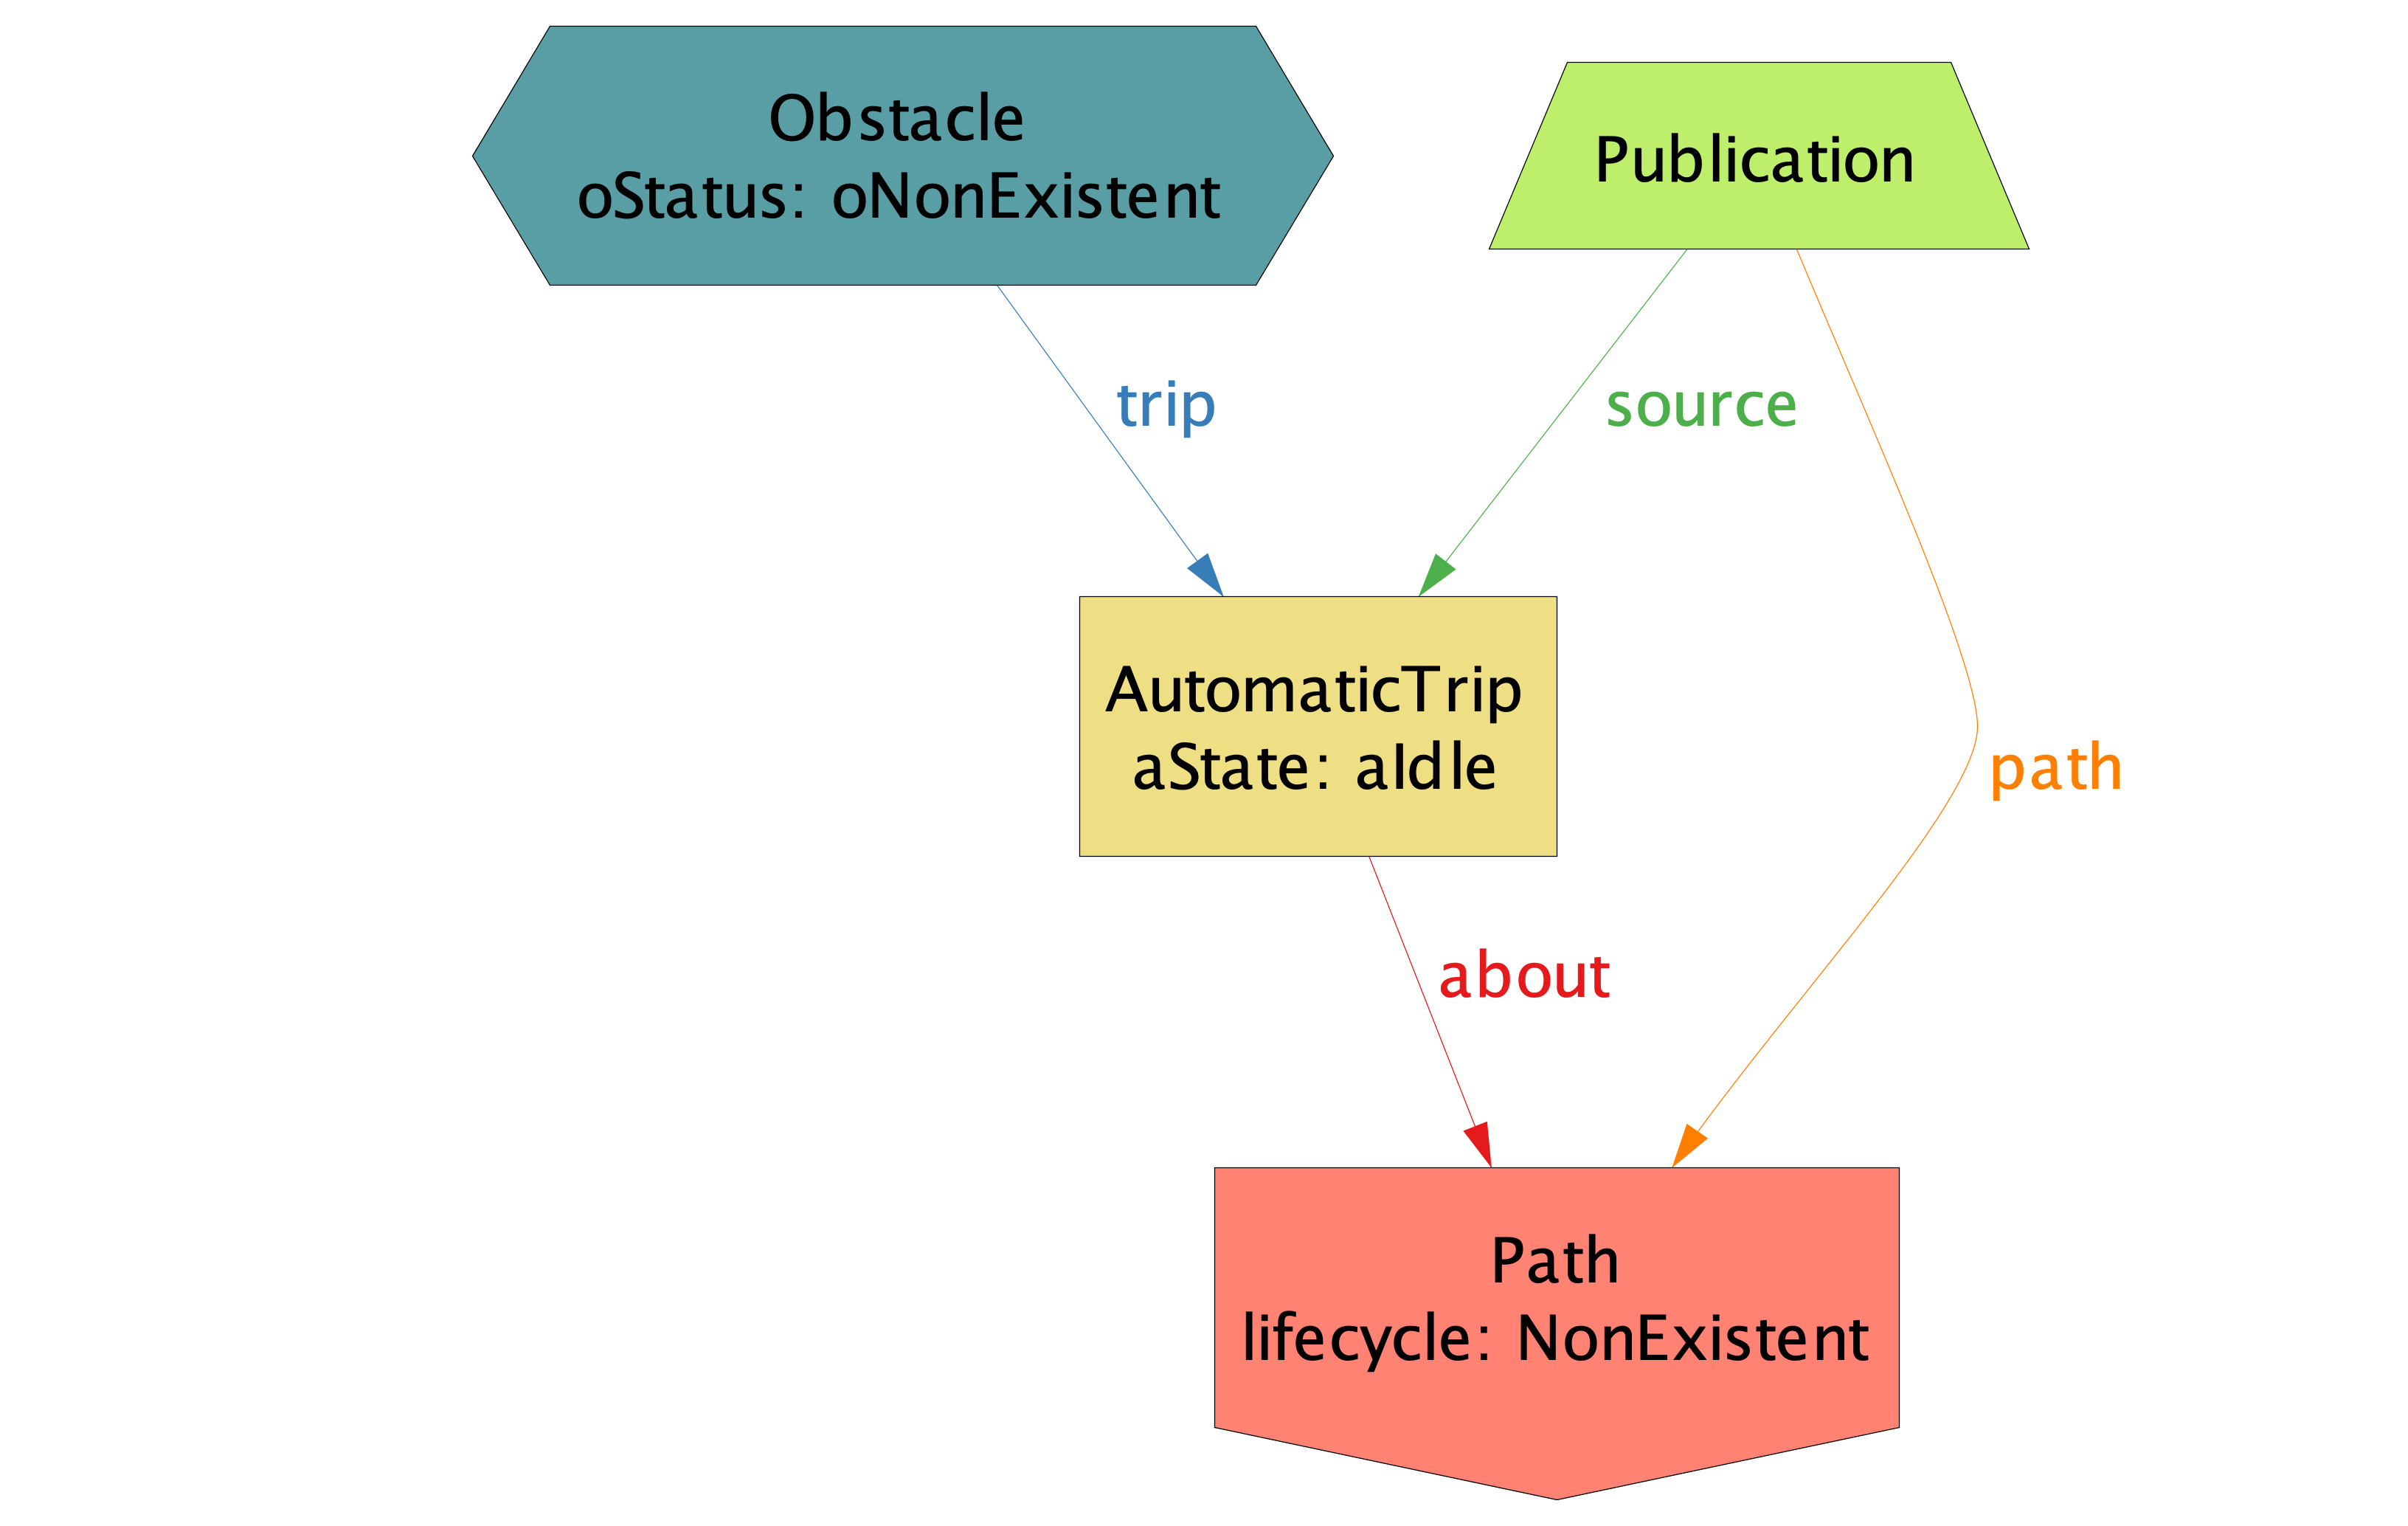
\includegraphics[width=0.8\textwidth]{diagrams/alloy_ex2/alloy_ex2_s0.png}
    \caption{Example 2 evolution: state 0}
    \label{fig:placeholder}
\end{figure}
\begin{figure}[H]
    \centering
    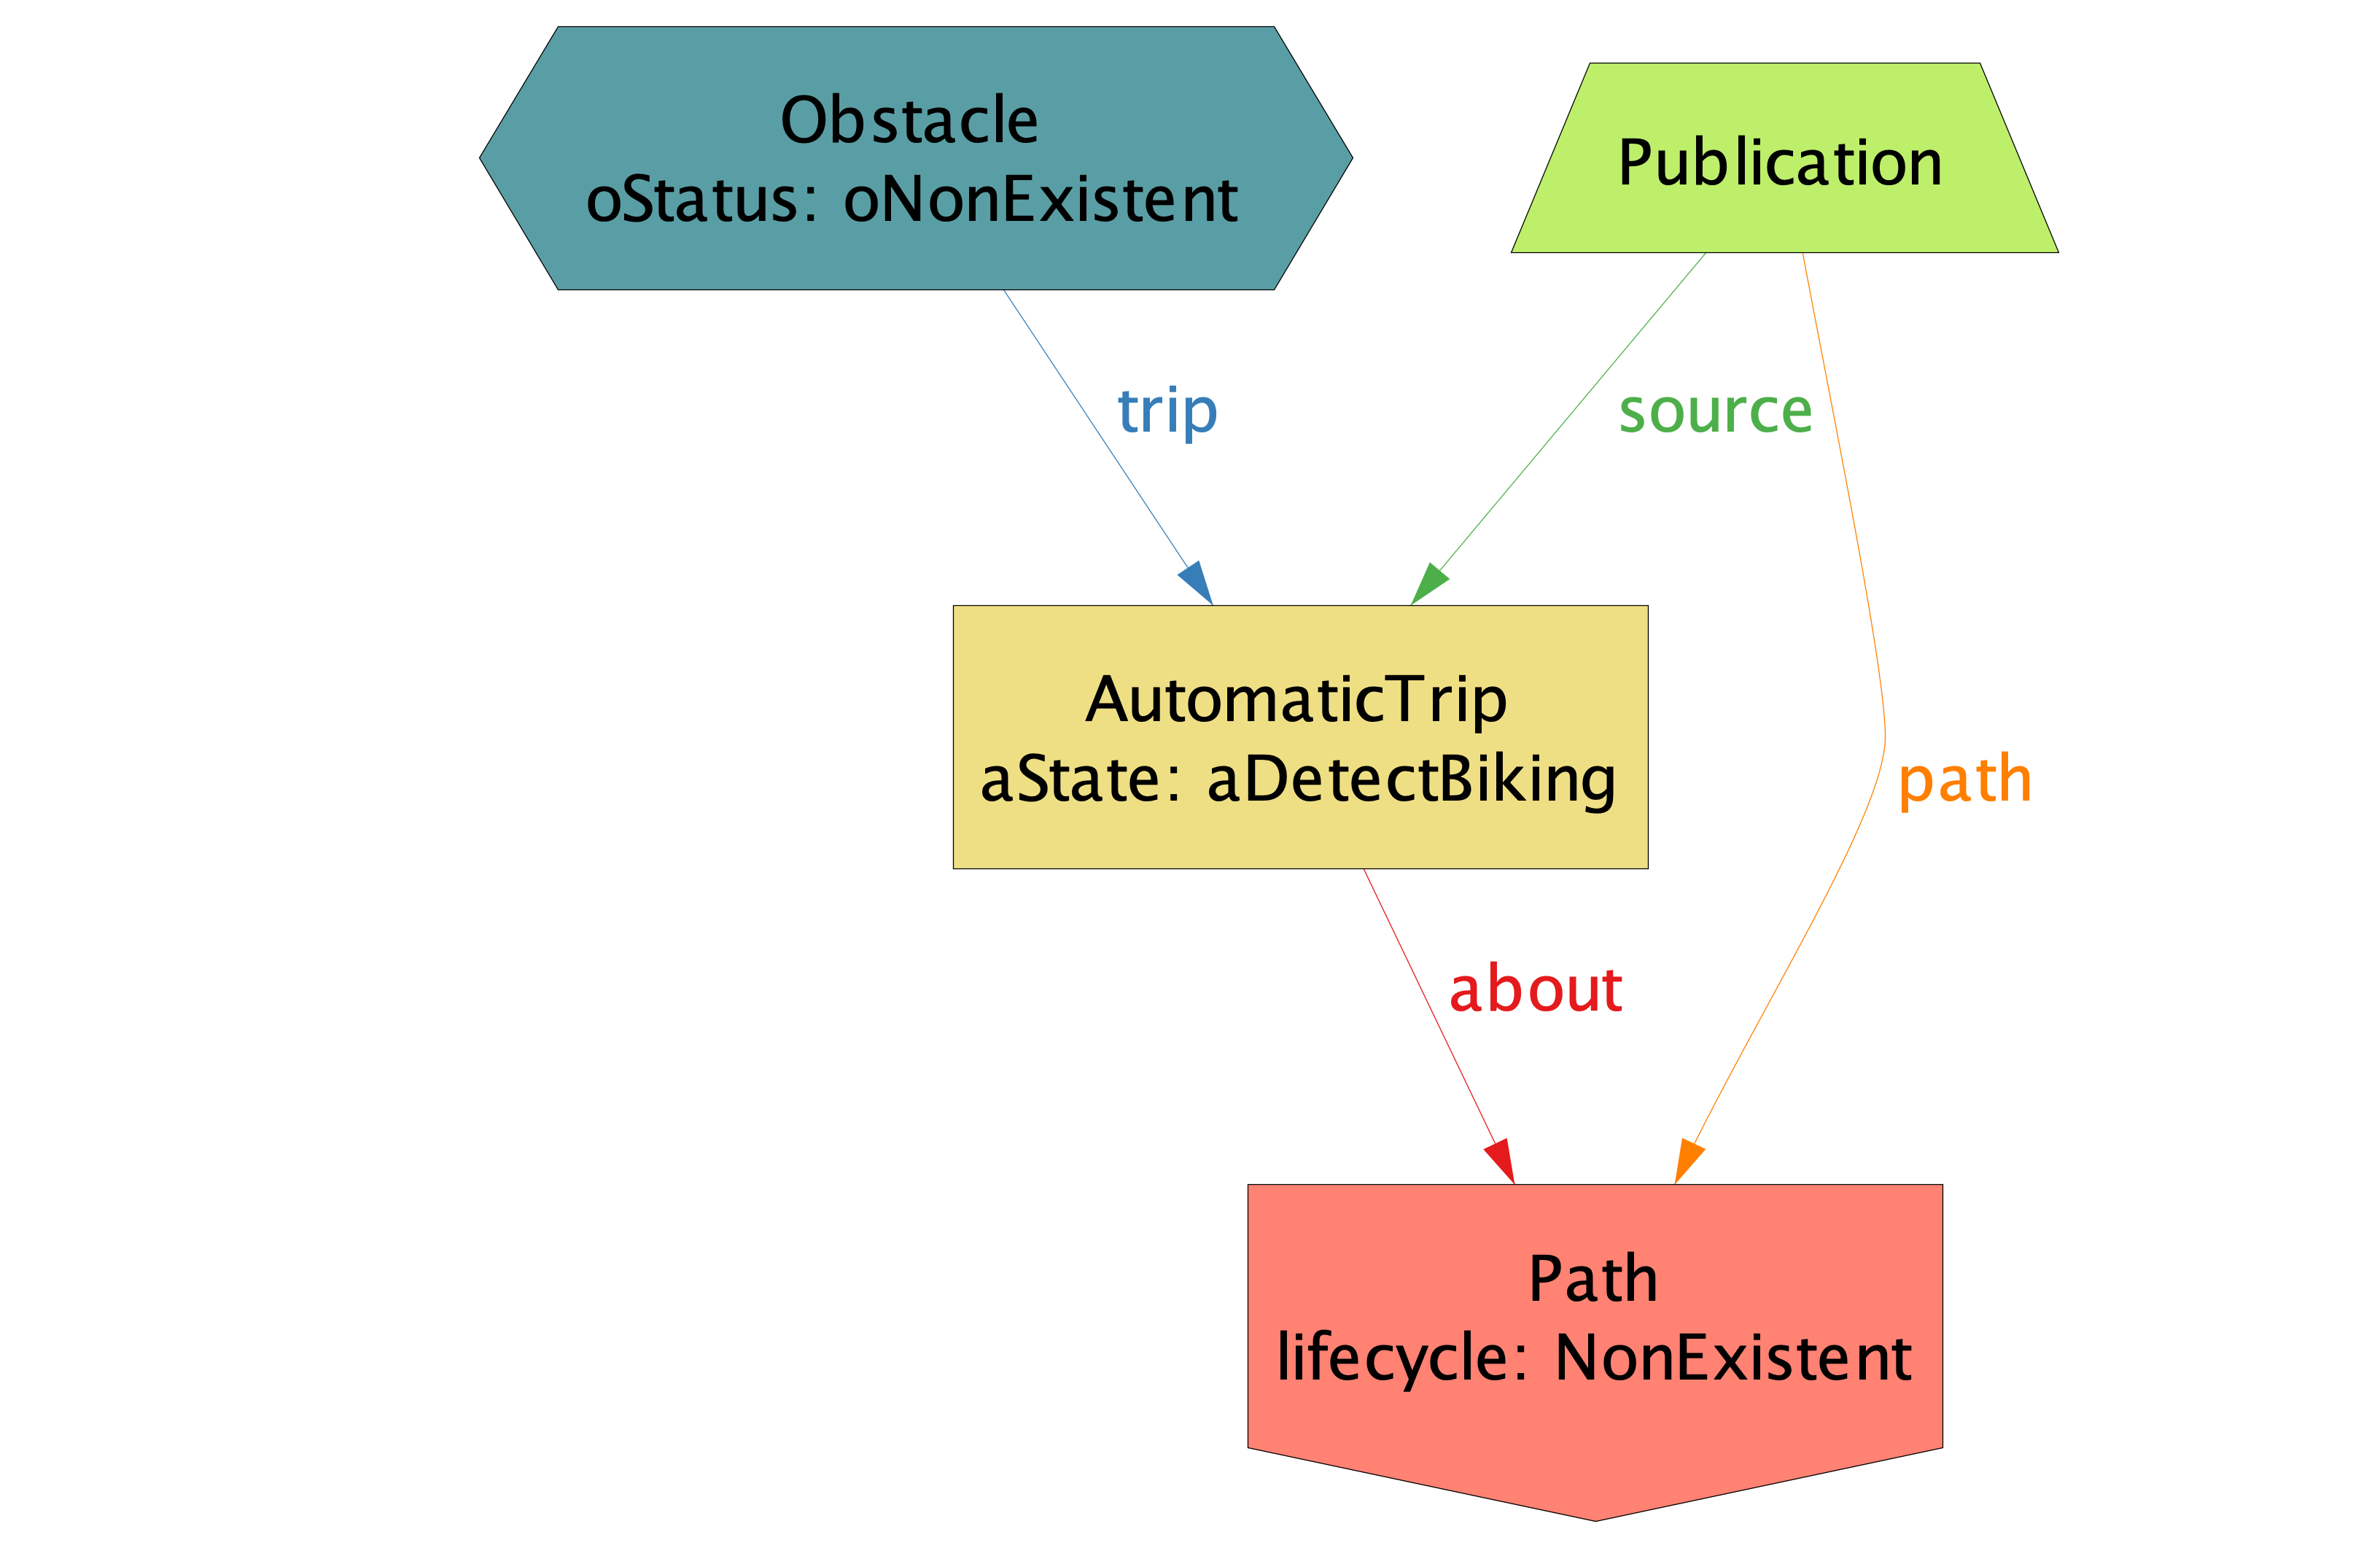
\includegraphics[width=0.8\textwidth]{diagrams/alloy_ex2/alloy_ex2_s1.png}
    \caption{Example 2 evolution: state 1}
    \label{fig:placeholder}
\end{figure}
\begin{figure}[H]
    \centering
    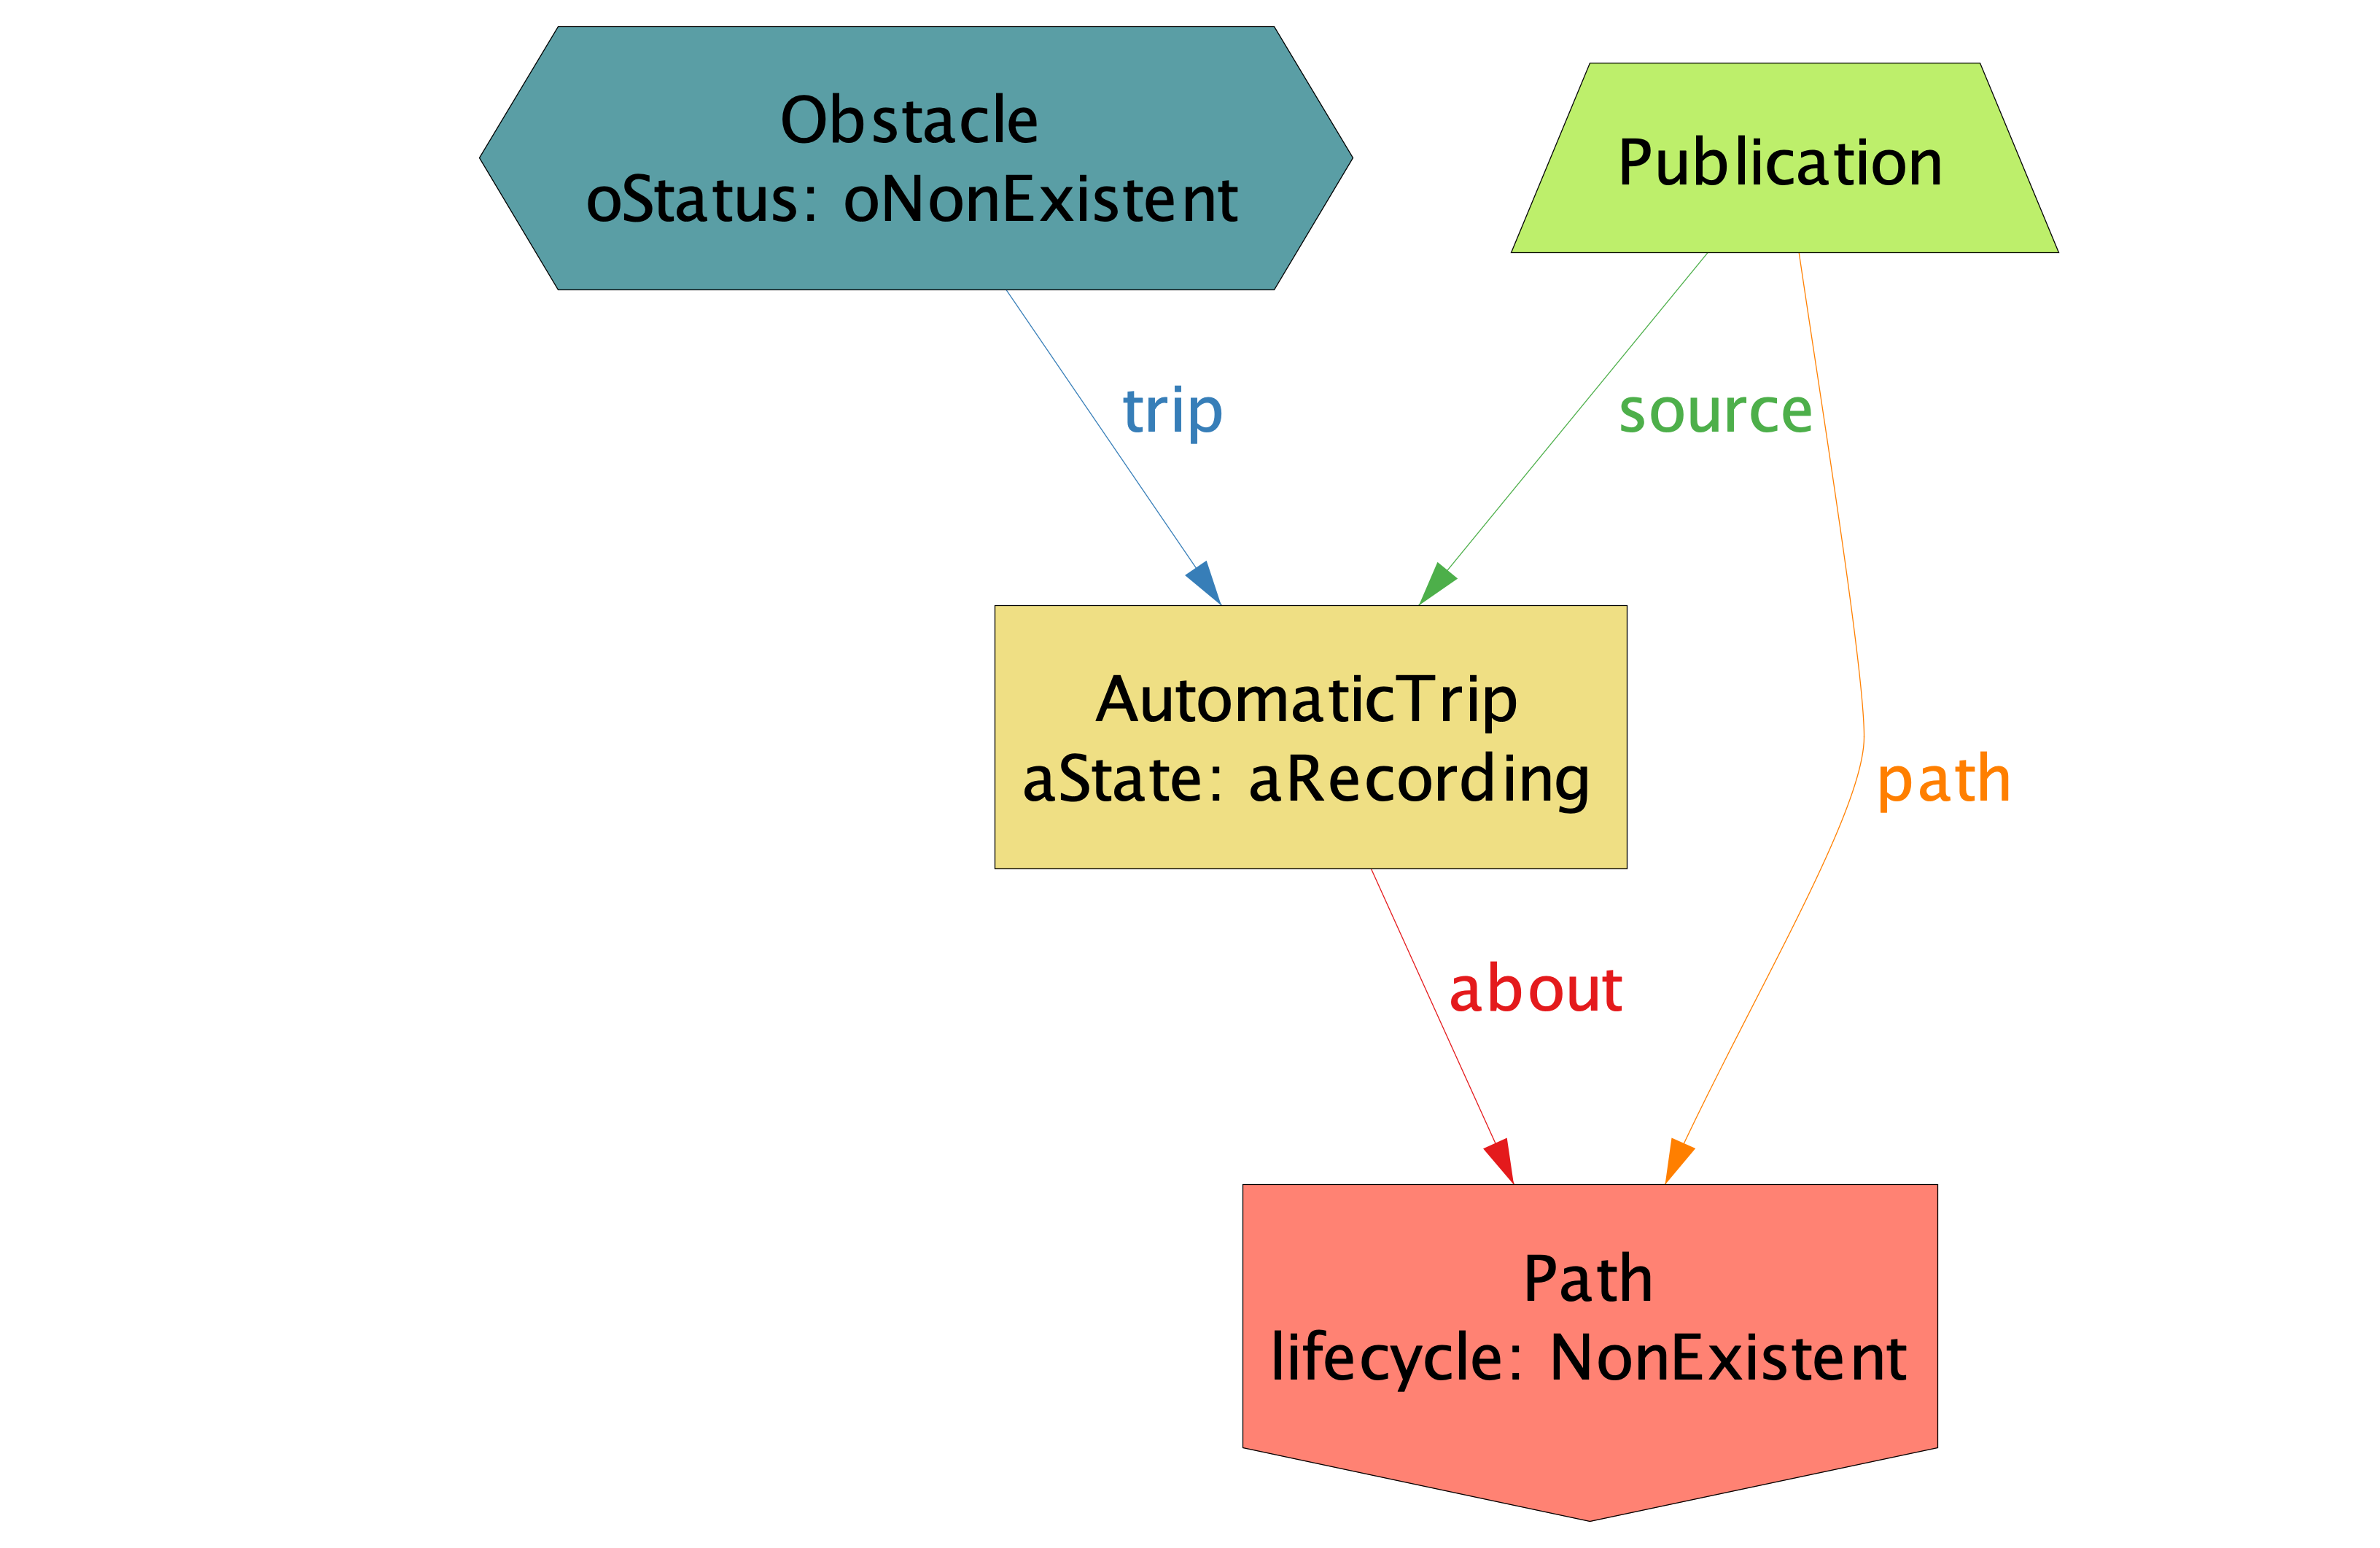
\includegraphics[width=0.8\textwidth]{diagrams/alloy_ex2/alloy_ex2_s2.png}
    \caption{Example 2 evolution: state 2}
    \label{fig:placeholder}
\end{figure}
\begin{figure}[H]
    \centering
    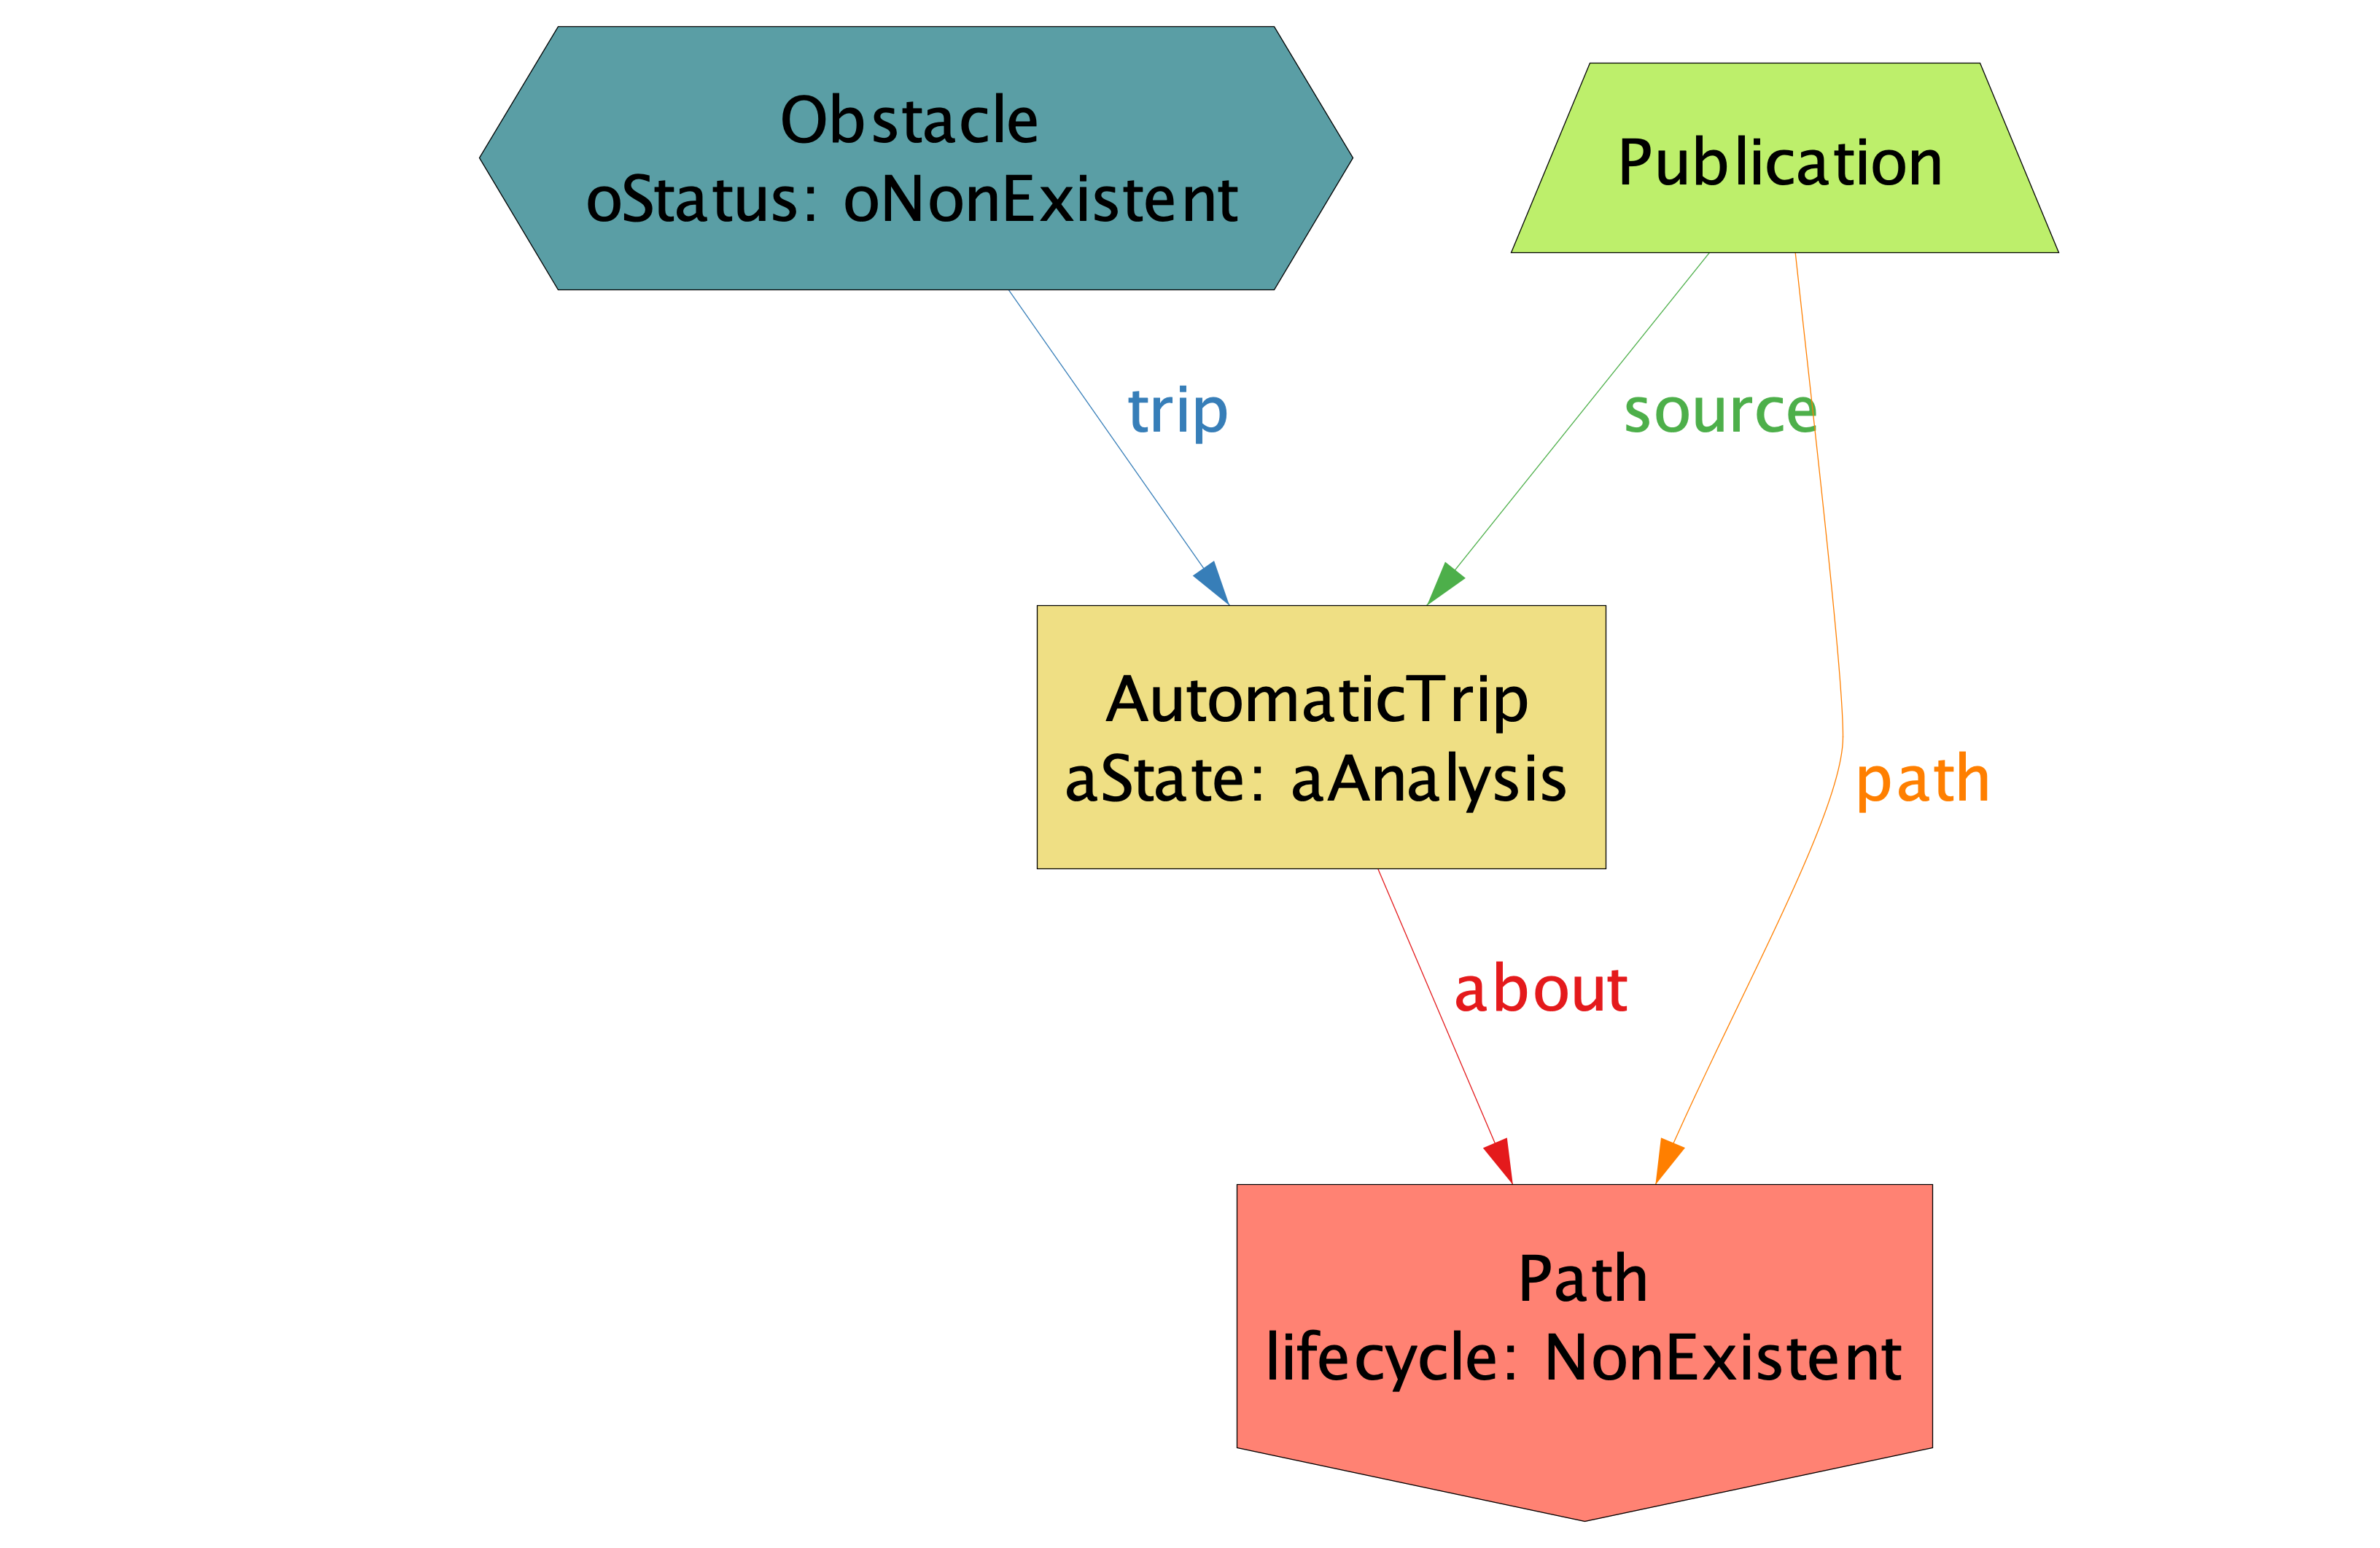
\includegraphics[width=0.8\textwidth]{diagrams/alloy_ex2/alloy_ex2_s3.png}
    \caption{Example 2 evolution: state 3}
    \label{fig:placeholder}
\end{figure}
\begin{figure}[H]
    \centering
    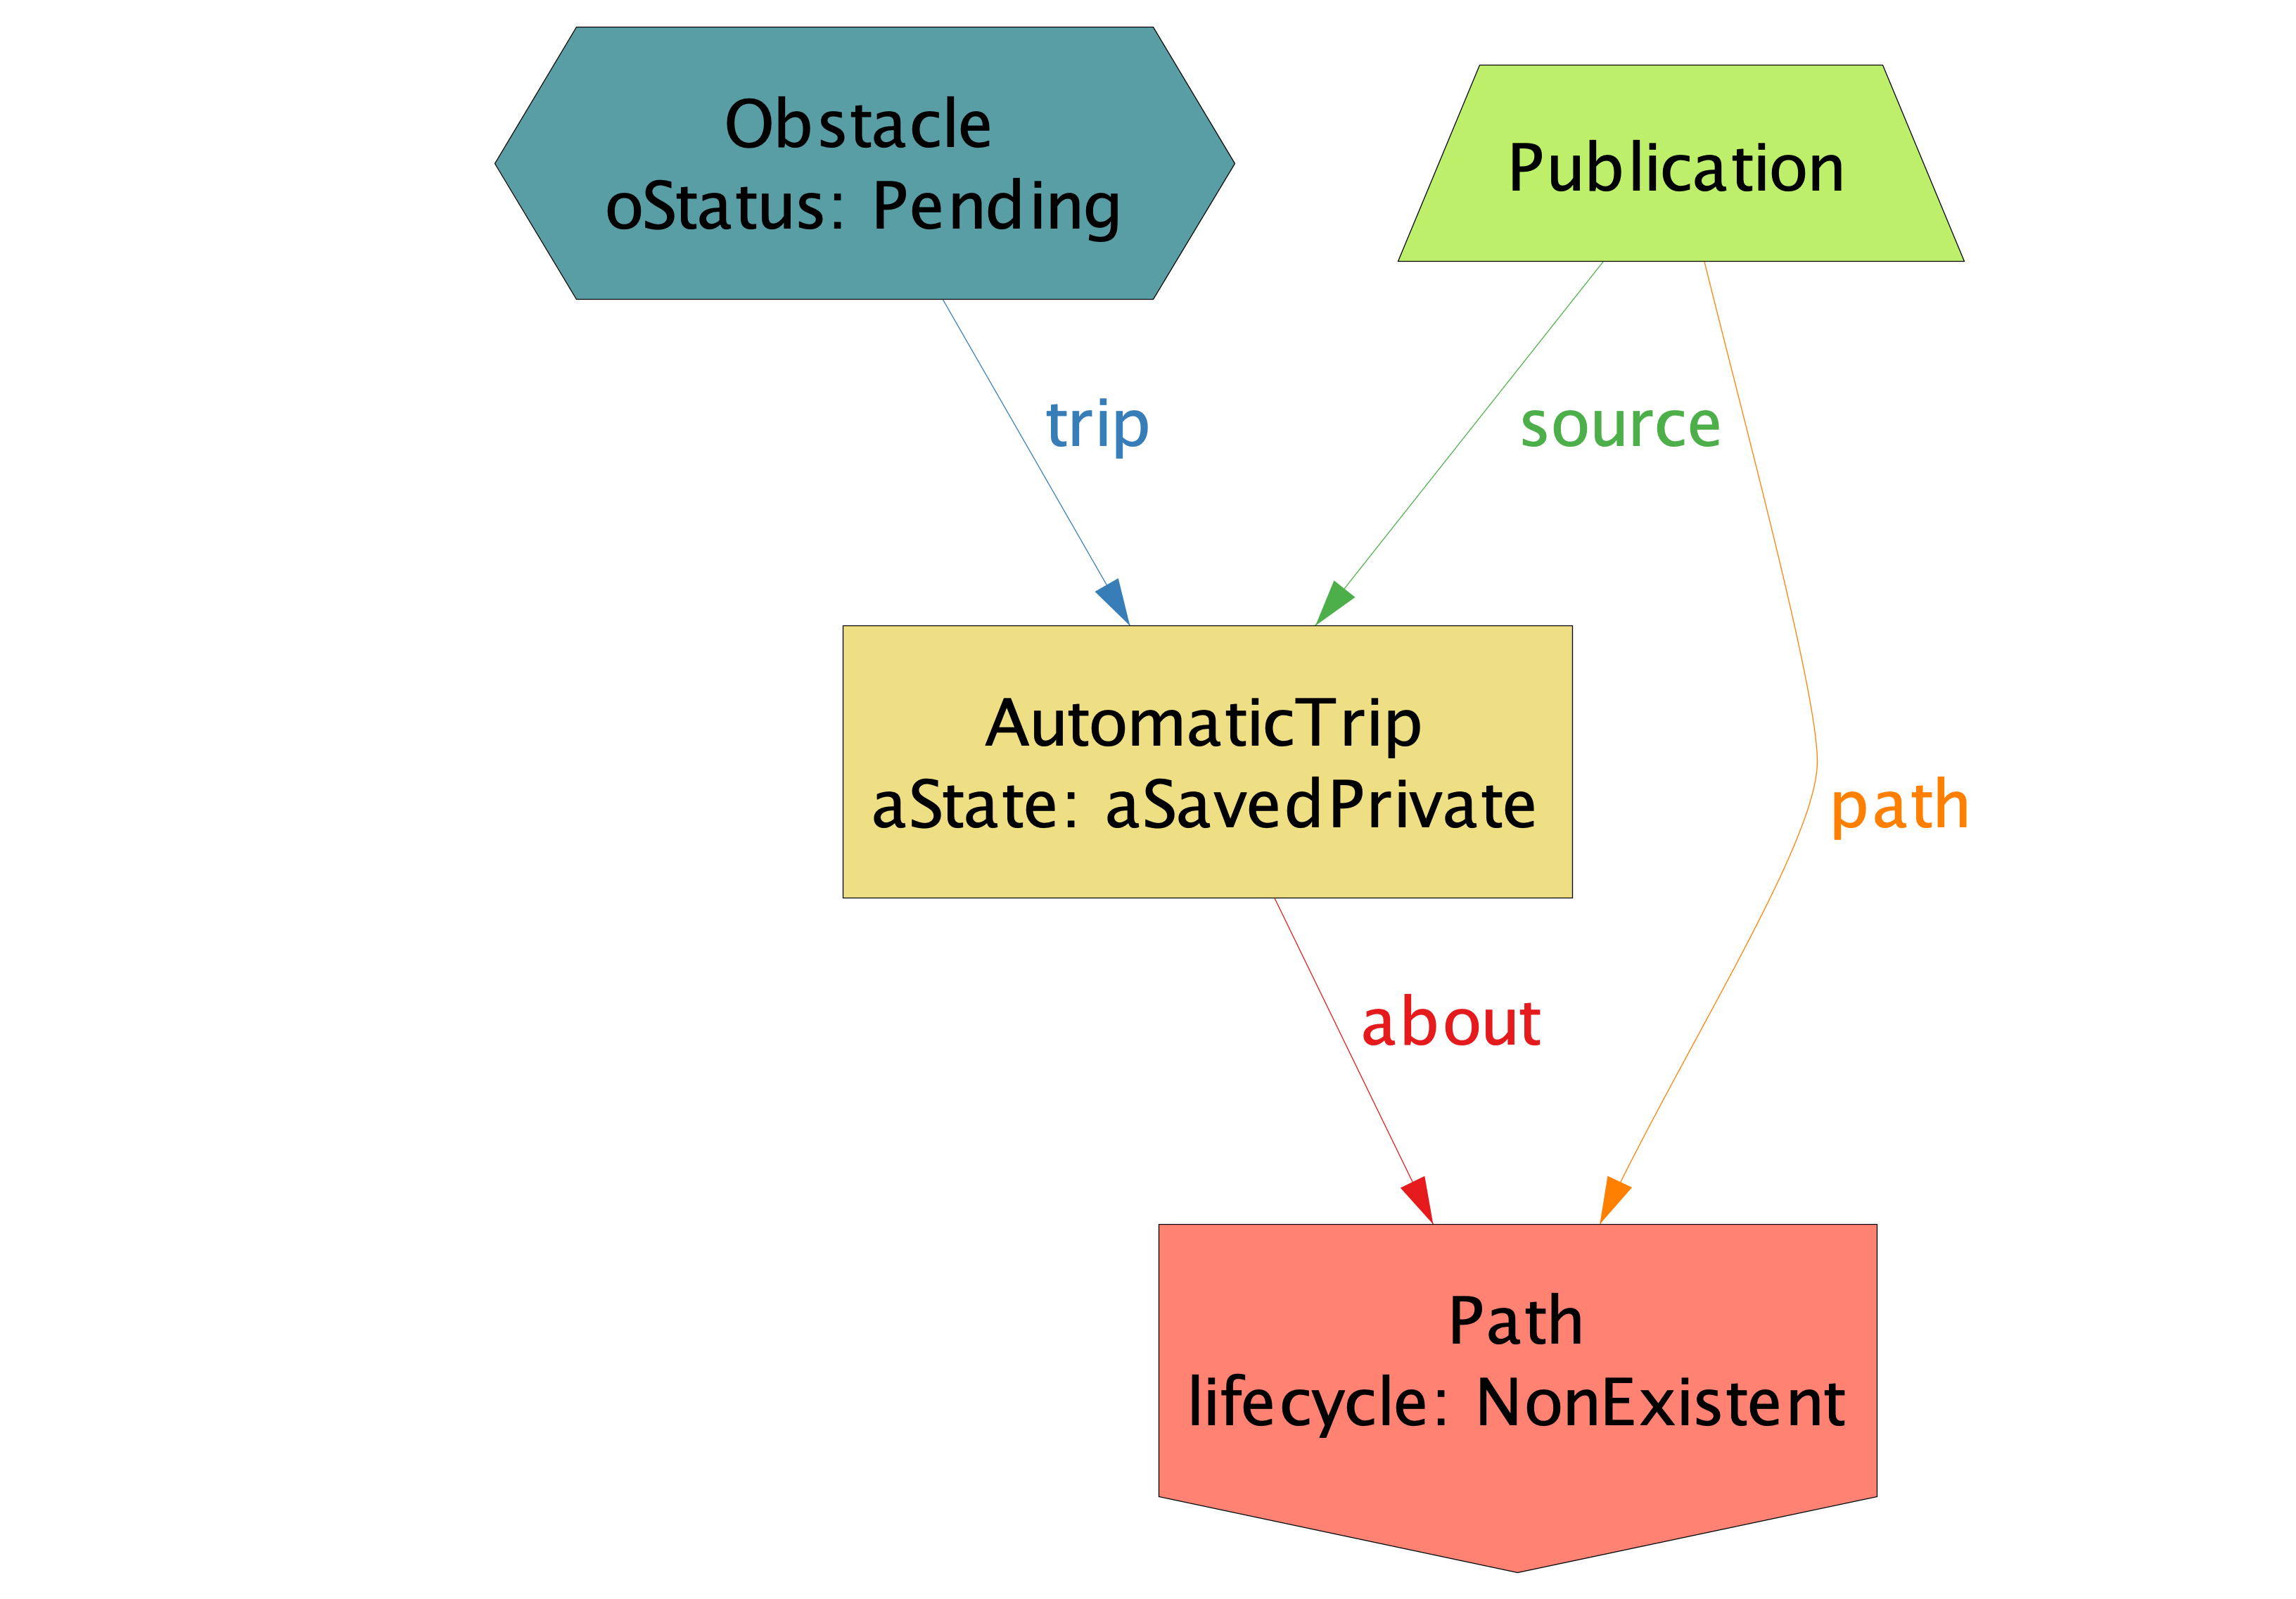
\includegraphics[width=0.8\textwidth]{diagrams/alloy_ex2/alloy_ex2_s4.png}
    \caption{Example 2 evolution: state 4}
    \label{fig:placeholder}
\end{figure}
\begin{figure}[H]
    \centering
    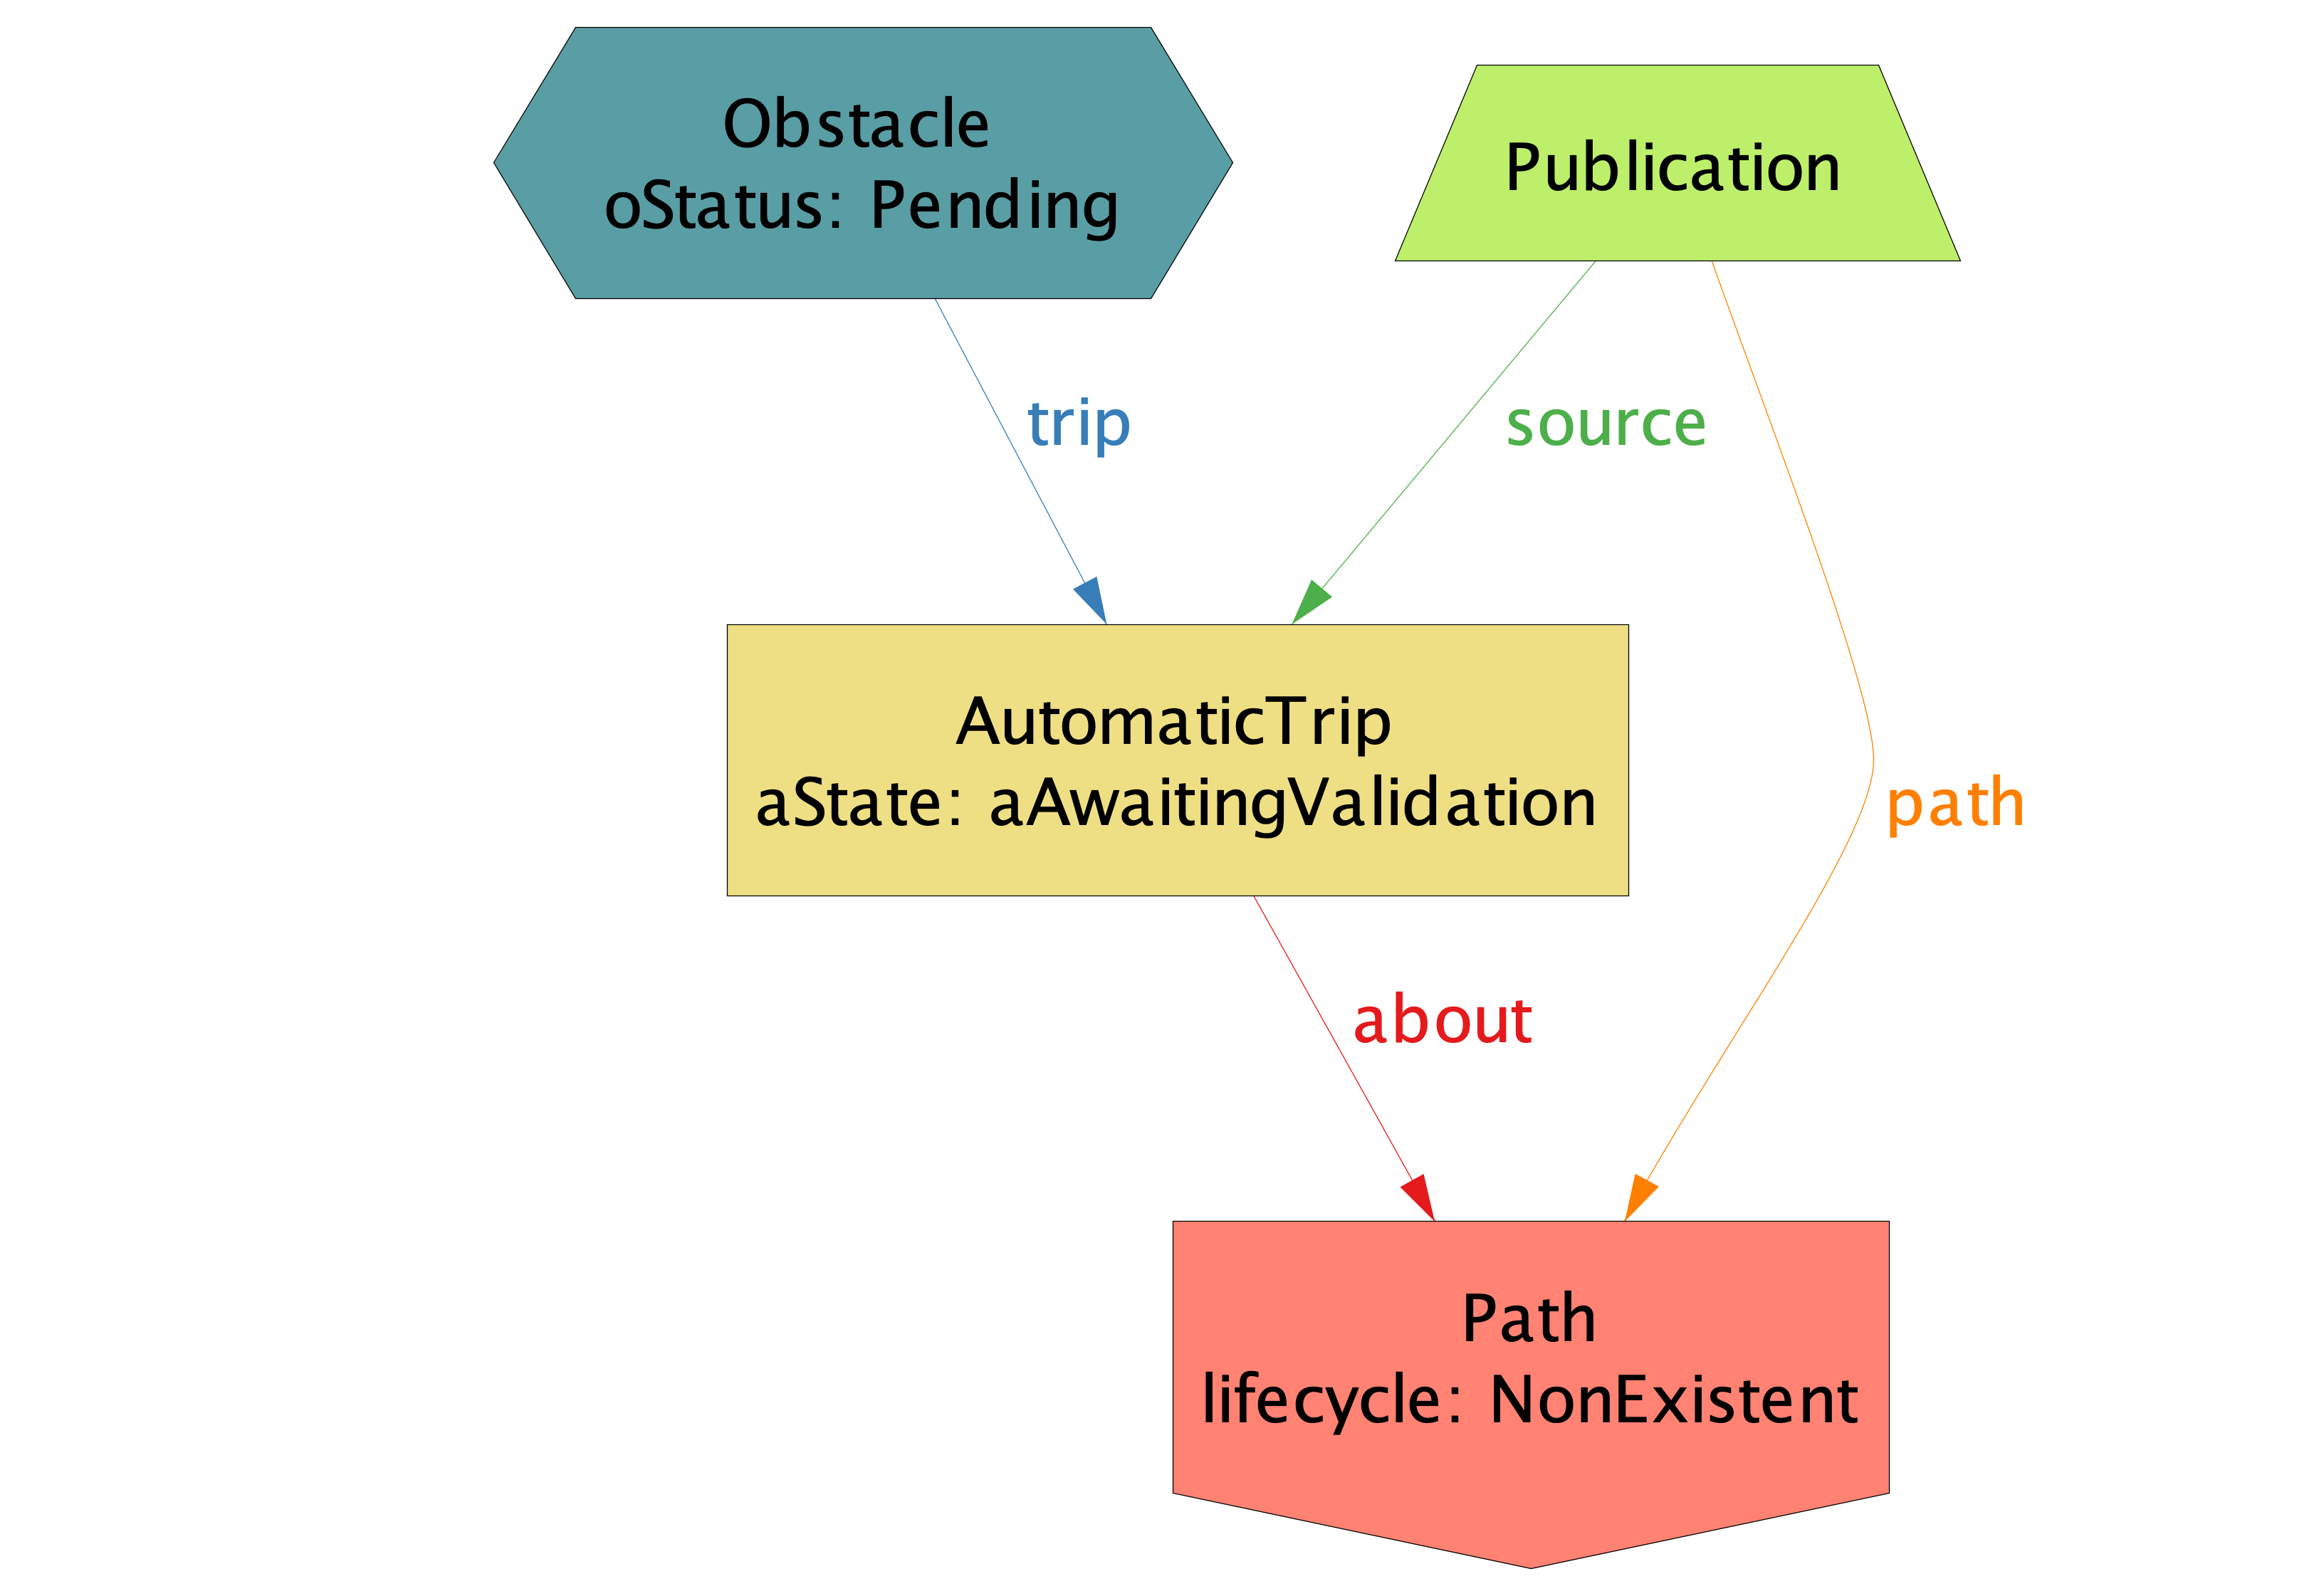
\includegraphics[width=0.8\textwidth]{diagrams/alloy_ex2/alloy_ex2_s5.png}
    \caption{Example 2 evolution: state 5}
    \label{fig:placeholder}
\end{figure}
\begin{figure}[H]
    \centering
    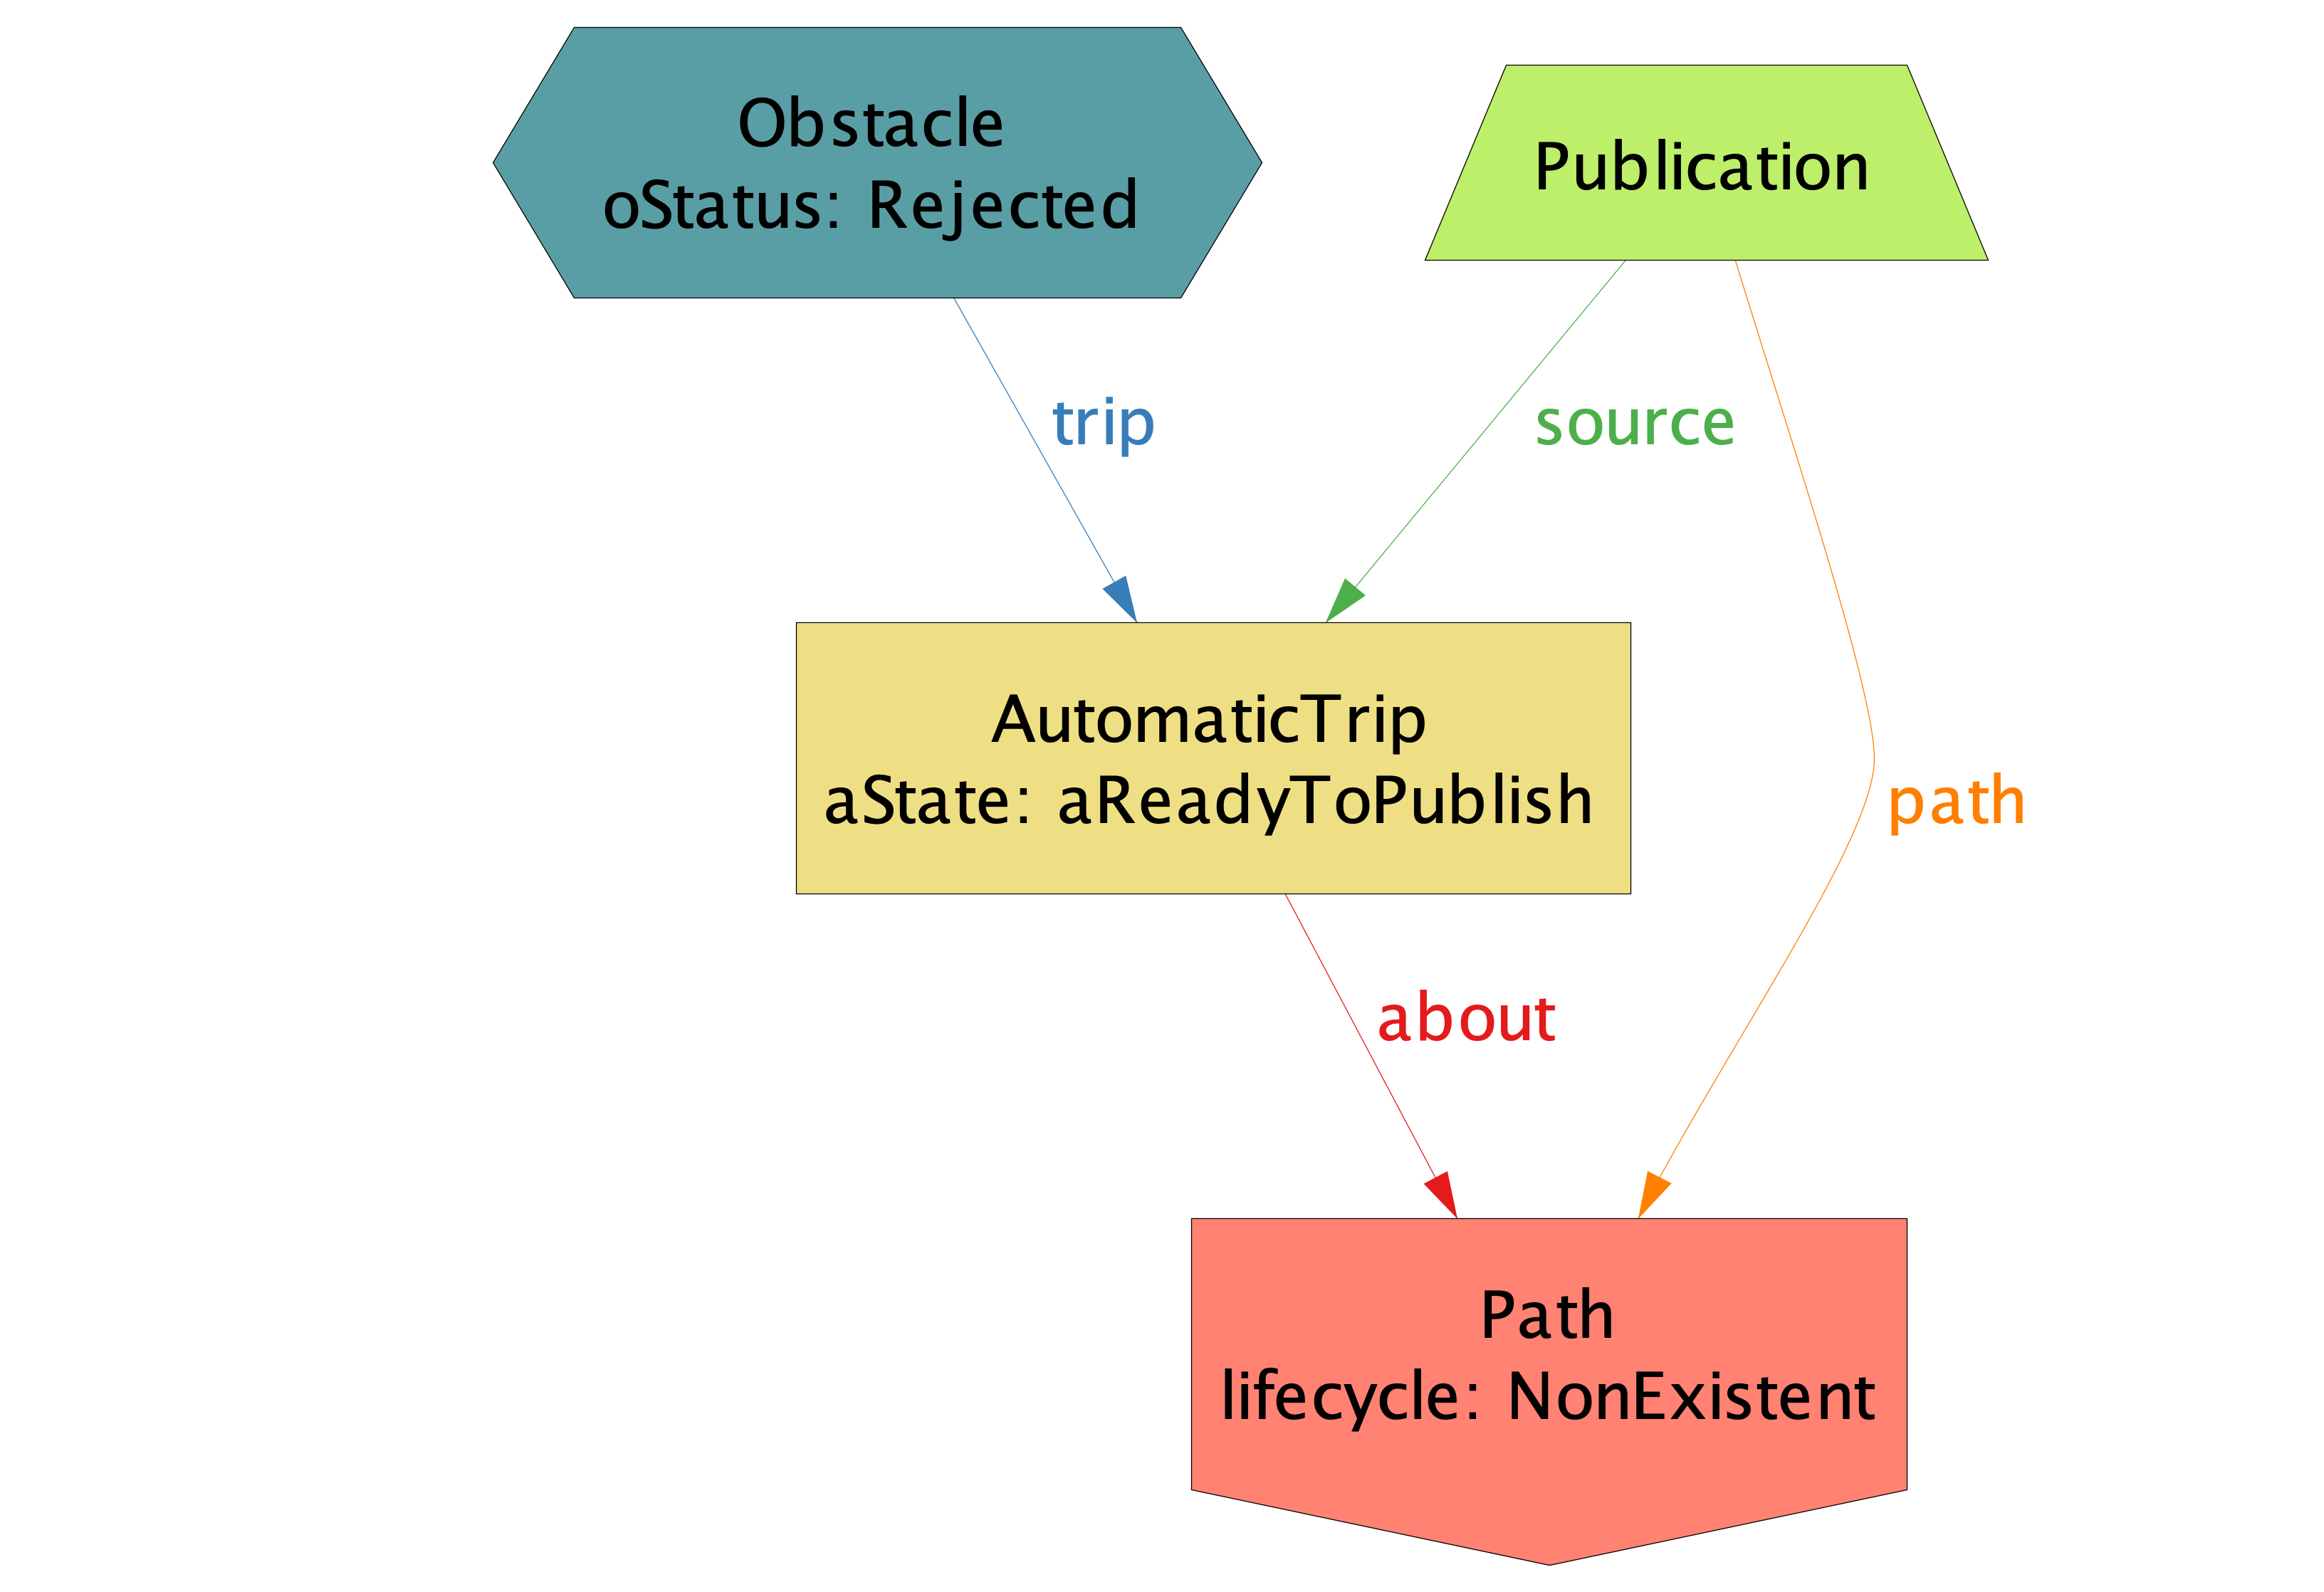
\includegraphics[width=0.8\textwidth]{diagrams/alloy_ex2/alloy_ex2_s6.png}
    \caption{Example 2 evolution: state 6}
    \label{fig:placeholder}
\end{figure}
\begin{figure}[H]
    \centering
    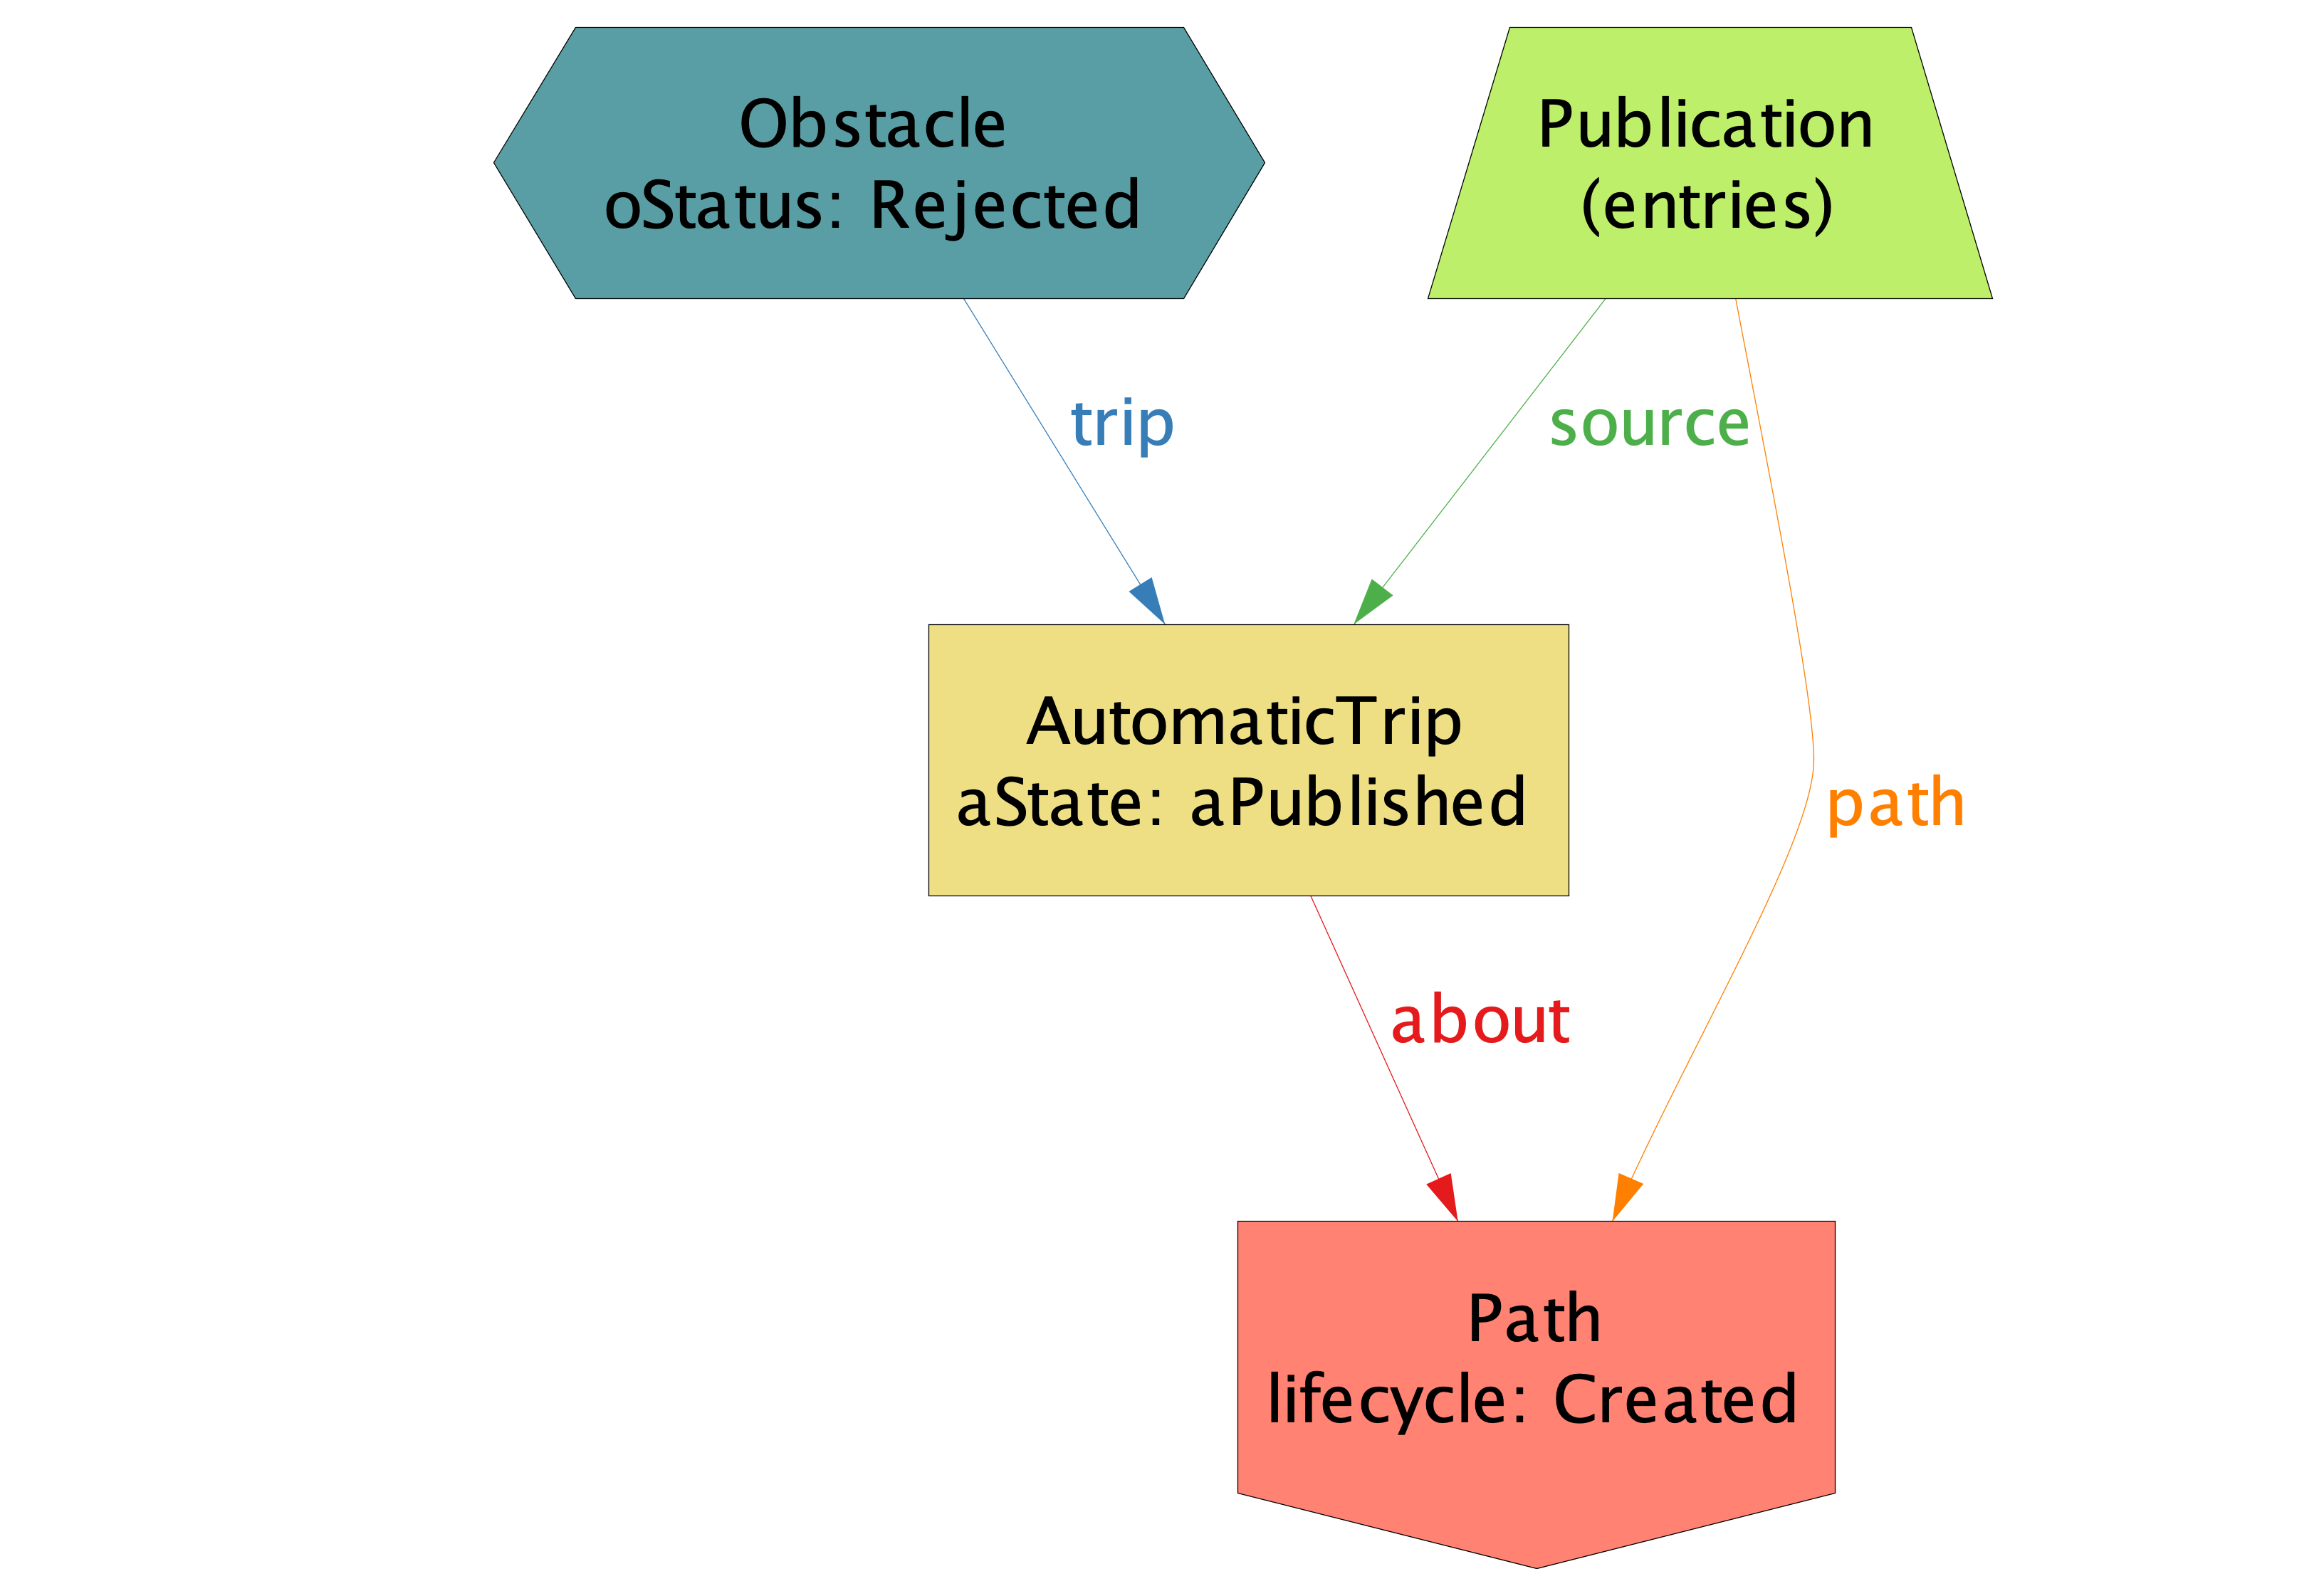
\includegraphics[width=0.8\textwidth]{diagrams/alloy_ex2/alloy_ex2_s7.png}
    \caption{Example 2 evolution: state 7}
    \label{fig:placeholder}
\end{figure}

\subsection{Assertions}
To test the code provided we used different assertions in order to ensure no edge
cases were present and verify global safety properties of the model.
\begin{lstlisting}[language=alloy]
// ManualTrip cannot be Published without passing through ReadyToPublish
assert manualTripPublishRequiresReady {
  all mt: ManualTrip | always (mt.mState = mPublished implies once (mt.mState = mReadyToPublish))
}

// AutomaticTrip cannot be Published if any pending obstacle exists
assert noPublishWithPendingObstacles {
  all at: AutomaticTrip | always (
    at.aState = aPublished implies
      no o: Obstacle | o.trip = at and o.oStatus = Pending
  )
}

// If a Path is PermanentlyClosed, it never changes status
assert permanentlyClosedIsAbsorbing {
  all p: Path | always (p.status = PermanentlyClosed implies after always (p.status = PermanentlyClosed))
}

// Deleting a trip cannot remove its anonymized contribution (log)
assert deletionDoesNotUndoPublication {
  all t: Trip |
    once (
      (t in ManualTrip and t.(ManualTrip <: mState) = mPublished) or
      (t in AutomaticTrip and t.(AutomaticTrip <: aState) = aPublished)
    )
    implies always (some e: Publication | e.source = t)
}

\end{lstlisting}